Στο κεφάλαιο αυτό παρουσιάζεται αναλυτικά η μελέτη της δυναμικής συμπεριφοράς ενός διακριτού συστήματος που αποτελεί παραλλαγή του γνωστού \emph{sine-sinh-sine} Χάρτη. Για επιλεγμένες τιμές της παραμέτρου του μποροεί να παρουσιάσει χαοτική συμπεριφορά όπως και φαινόμενα που σχετίζονται με τη μη-γραμμική δυναμική. Για την μελέτη χρησιμοποιήθηκαν τα διαγράμματα διακλάδωσης, οι εκθέτες Lyapunov και οι απεικονίσεις της τιμής \(x_i\) σε συνάρτηση με  την τιμή \(x_{i+1}\).

Ο \emph{sine-sinh-sine} Χάρτης που αποτέλεσε τη βάση του προτεινόμενου σε αυτή την ενότητα, χάρτη, περιγράφεται από την παρακάτω εξίσωση:

\begin{equation}
	x_i=k*\sin(\pi*\sinh(\pi*\sin(\pi* x_{i-1})))
	\label{f:x2}
\end{equation}


Στην εξίσωση (\ref{f:x2}) προστέθηκε ένας σταθερός όρος \emph{q}. Έτσι προέκυψε η προτεινόμενη παραλλαγή του Λογιστικού Χάρτη,

\begin{equation}
	x_i=k*\sin(k*\sinh(q*\sin(2 * x_{i-1})))
	\label{f:x3}
\end{equation}
όπου \emph{k}, \emph{q} : παράμετροι.\\

Για την εύρεση της δυναμικής συμπεριφοράς του συστήματος (3.2) εξετάστηκε μια περιοχή τιμών των συγκεκριμένων παραμέτρων. Πιο συγκεκριμένα, στη μελέτη που πραγματοποιήθηκε η αρχική συνθήκη του συστήματος $x_0 =0.1$ παρέμεινε  σταθερή, ενώ η τιμή της παραμέτρου \emph{q} μεταβαλλόταν στο διάστημα $[-0.3,-0.5]$ με βήμα $0.2$. Έτσι, για κάθε περίπτωση παράχθηκαν το διάγραμμα διακλάδωσης, το διάγραμμα των εκθετών Lyapunov και το διάγραμμα της τιμής \(x_i\) σε συνάρτηση με  την τιμή \(x_{i+1}\), τα οποία παρουσιάζονται και αναλύονται στη συνέχεια.\\


\vspace{\fill}

\section{Για \emph{q} = -0.3}


Στo Σχ. \ref{f:g44} παρατίθεται τα διάγραμμα διακλάδωσης του συστήματος (\ref{f:x3}), ως προς την παράμετρο \emph{k}, για $q =- 0.3$. 
Στον πίνακα \ref{tab:abc10} φαίνεται η πορεία του συστήματος και για ποιες τιμές της παραμέτρου \emph{k} το σύστημα εμφανίζει περιοδική ή χαοτική συμπεριφορά, σύμφωνα με το διάγραμμα διακλάδωσης του Σχ. \ref{f:g44}. Επίσης παρατηρείται εσωτερική κρίση ελκυστών για διάφορες τιμές του \emph{k} (2.27, 2.31, 2.43, 2.671, 2.76, 2.935, 3.293, 3.48, 3.629, 3.79), όπως και το φαινόμενο της υστέρησης το οποίο φαίνεται στο διάγραμμα διακλάδωσης του Σχ. \ref{f:g44}, στην μεταπήδηση του συστήματος από χαοτική συμπεριφορά σε \emph{περίοδο - 1} και \emph{περίοδο - 2}. Οι αντίστοιχες τιμές του \emph{k} για αυτά τα σημεία του διαγράμματος υπάρχουν στο Πίνακα \ref{tab:abc10}, όπως και τα αντίστοιχα Σχ. \ref{f:k246}, \ref{f:k247} των διαγραμμάτων της τιμής \(x_i\) σε συνάρτηση με την τιμή \(x_{i+1}\). Από τα παραγόμενα σχήματα προκύπτει αριθμός σημείων αντίστοιχος με την περίοδο του συστήματος.

Τέλος, στο Σχ. \ref{f:g45} παρατίθεται το διάγραμμα των εκθετών Lyapunov για τιμές του \emph{k} στο ίδιο διάστημα τιμών $[0, 4.2]$. Οι τιμές του Πίνακα \ref{tab:abc10} που έχουν περιοδική συμπεριφορά αντιστοιχούν σε τιμές του διαγράμματος του Σχ. \ref{f:g44} όπου o εκθέτης Lyapunov είναι συνεχώς αρνητικός, γεγονός που επιβεβαιώνει την συμπεριφορά του. Ενώ για τις υπόλοιπες τιμές ο θετικός εκθέτης Lyapunov υποστηρίζει την χαοτική του συμπεριφορά, όπως έγινε φανερό και από το διάγραμμα διακλάδωσης.\\\\





\begin{table}[ht]
	\centering
	\caption{ Συμπεριφορά του υπό μελέτη συστήματος για διάφορες τιμές του \emph{k}, για $q=-0.3$ }
	\label{tab:abc10}
	\begin{tabular}{l | l}
		Παράμετρος k & Συμπεριφορά \\
		\hline
		0.25 &  Περίοδος -  1 \\
		1.287 &  Περίοδος -  2 \\
		2.17& Περίοδος -  4 \\
		2.2& Περίοδος -  8 \\
		2.21 & Xάος \\
		2.27& Περίοδος - 10 \\
		2.272& Χάος \\
		2.31& Περίοδος - 6 \\
		2.32 &  Χάος \\
		2.43 &  Περίοδος -  3 \\
		2.435 &  Χάος \\
		2.671 &  Περίοδος -  3\\
		2.672 & Περίοδος - 6\\
		2.675 & Χάος\\
		2.76 &Περίοδος - 6 \\
		2.77& Χάος\\
		2.935 & Περίοδος -  1\\
		3.14& Περίοδος - 2\\
		3.22 & Περίοδος -  4\\
		3.238 & Περίοδος -  8\\
		3.24 & Χάος\\
		3.293 & Περίοδος -  3\\
		3.294 & Περίοδος -  6\\
		3.295 & Χάος\\
		3.48& Περίοδος -  4\\
		3.49 & Χάος\\
		3.629 &  Περίοδος -  2\\
		3.632 &  Περίοδος -  4 \\
		3.643 & Χάος\\
		3.79 & Περίοδος -  4\\
		3.8 & Χάος\\
		4.09 & Περίοδος -  2\\
		
		
	\end{tabular}
	
\end{table}


\begin{figure}[ht]
	\centering
	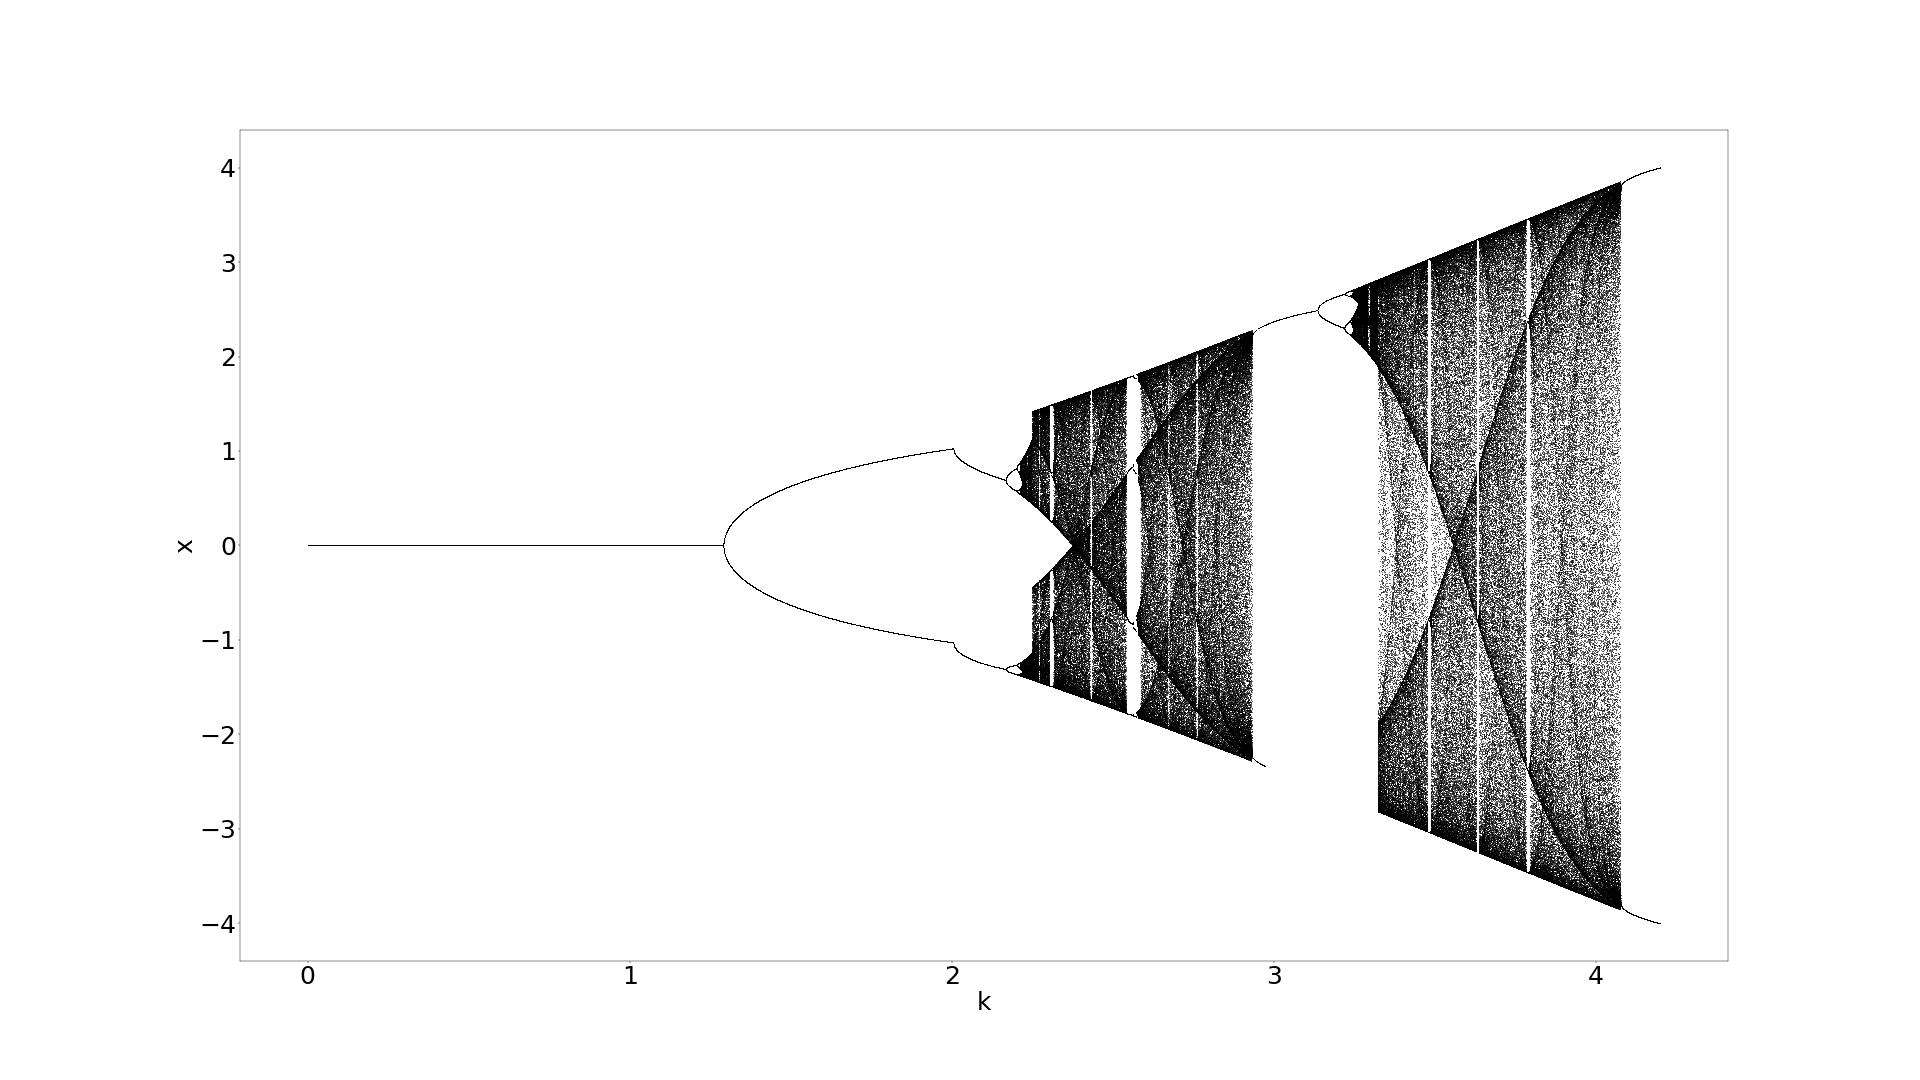
\includegraphics[width=1\linewidth]{LateX images/sine q=-0.3/g1}
	\caption{Διάγραμμα διακλάδωσης, για $q=-0.3$.}
	\label{f:g44}
\end{figure}


\begin{figure}[ht]
	\centering
	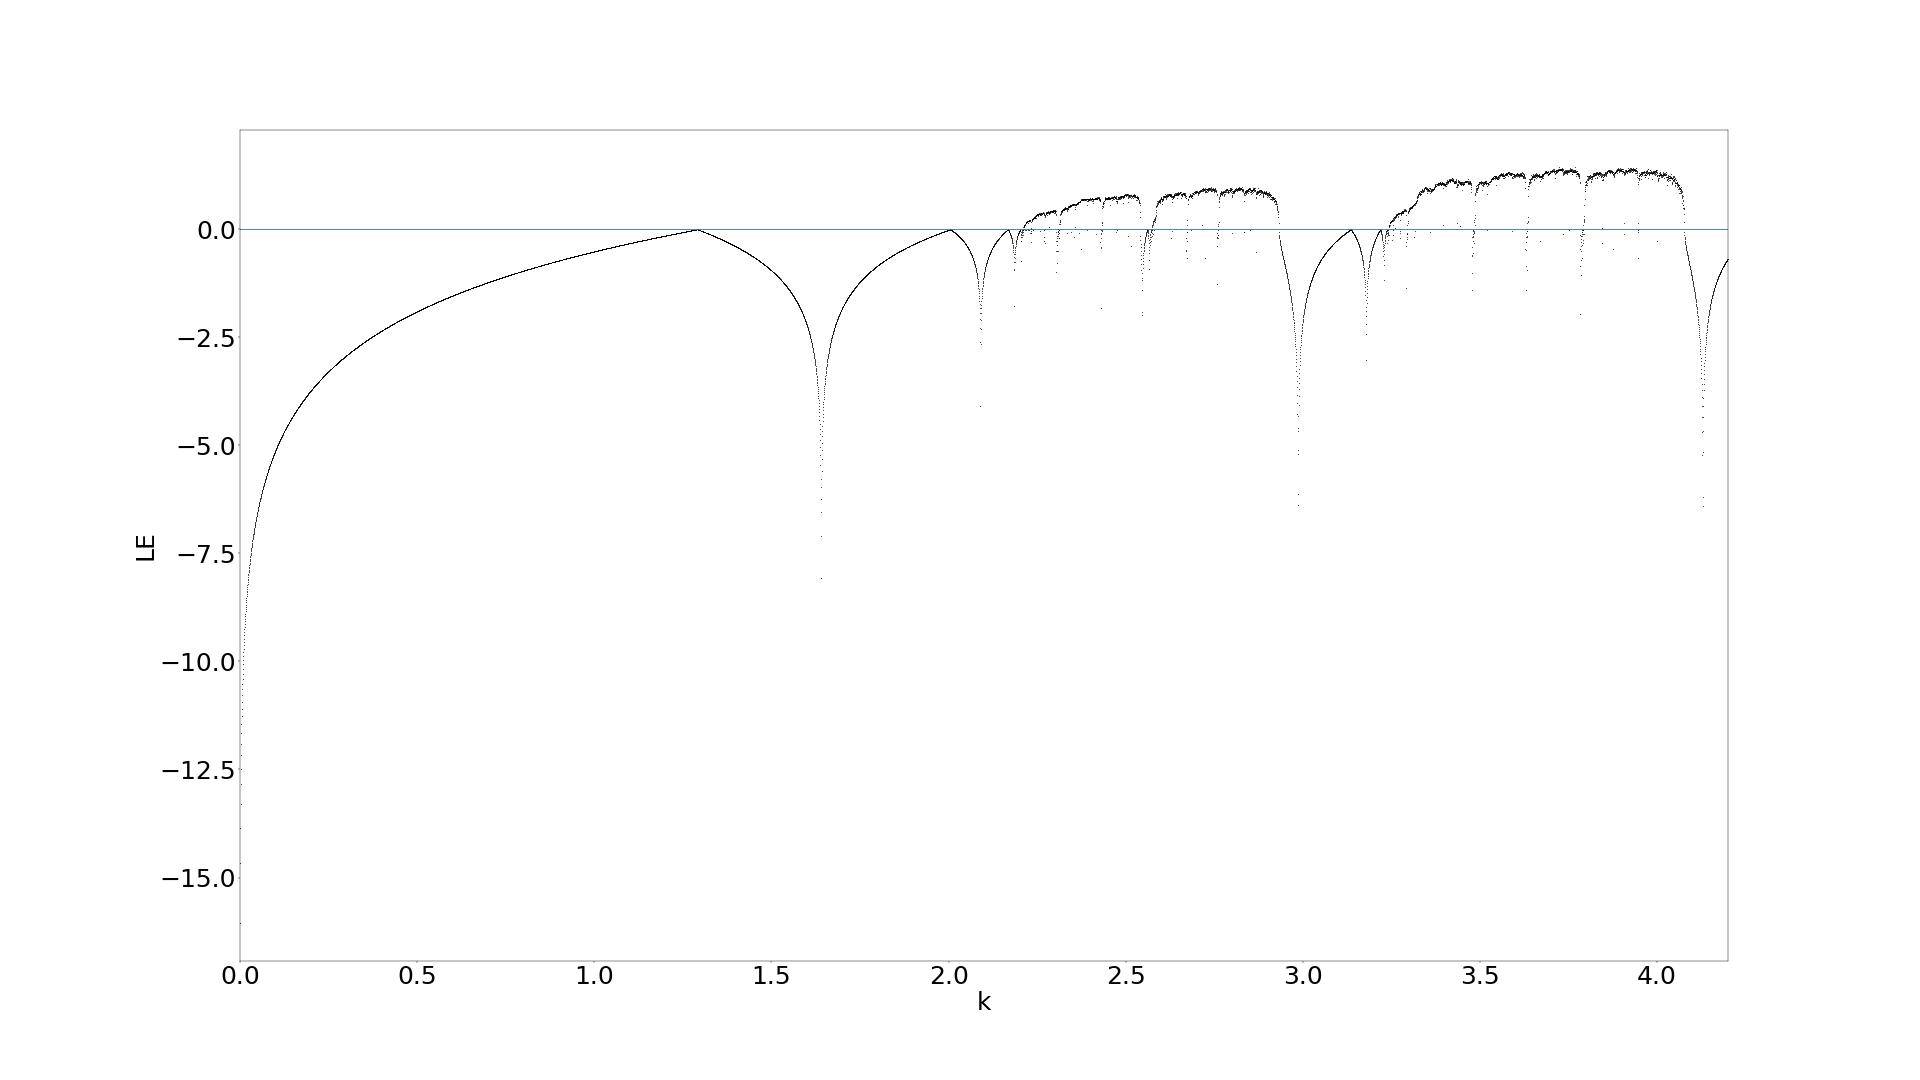
\includegraphics[width=1\linewidth]{LateX images/sine q=-0.3/g2}
	\caption{Διάγραμμα των εκθετών Lyapunov σε συνάρτηση με την παράμετρο \emph{k}, για $q=-0.3$.}
	\label{f:g45}
\end{figure}



\begin{figure}[ht]
	\centering
	\begin{subfigure}[b]{0.4\textwidth}
		\centering
		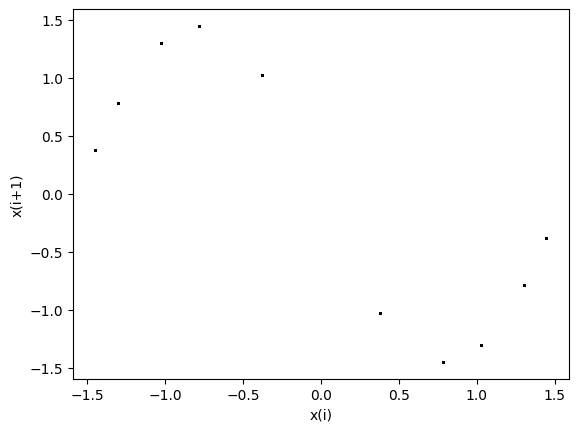
\includegraphics[width=\textwidth]{LateX images/sine q=-0.3/g3}
		\caption{Για $k=2.27$}
		\label{f:k116}
	\end{subfigure}
	\hfill
	\begin{subfigure}[b]{0.4\textwidth}
		\centering
		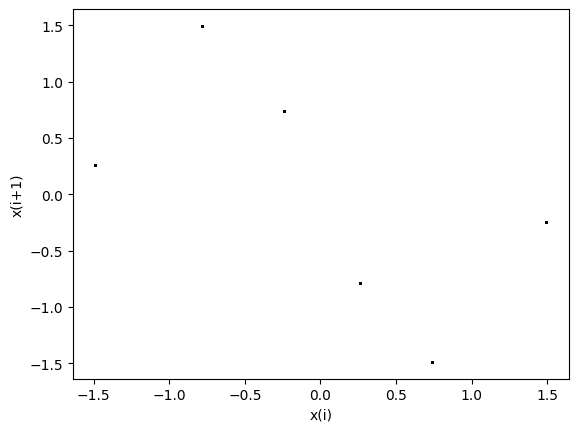
\includegraphics[width=\textwidth]{LateX images/sine q=-0.3/g4}
		\caption{Για $k=2.31$}
		\label{f:k117}
	\end{subfigure}
	\hfill
	\begin{subfigure}[b]{0.4\textwidth}
		\centering
		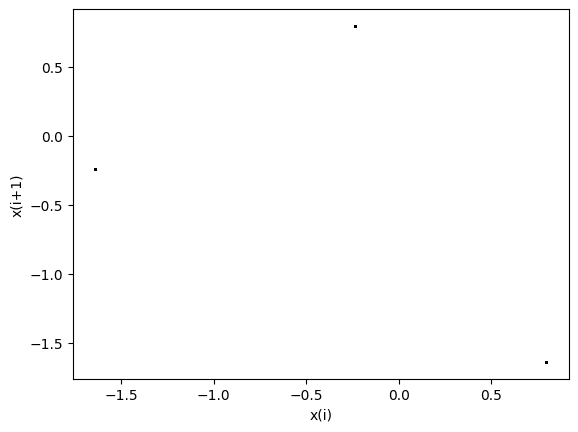
\includegraphics[width=\textwidth]{LateX images/sine q=-0.3/g5}
		\caption{Για $k=2.43$}
		\label{f:k118}
	\end{subfigure}
	\hfill
	\begin{subfigure}[b]{0.4\textwidth}
		\centering
		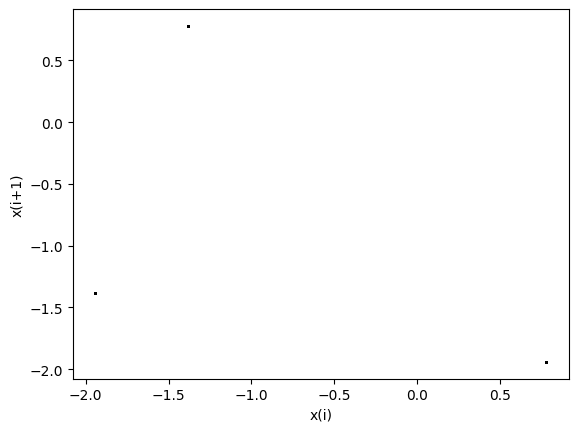
\includegraphics[width=\textwidth]{LateX images/sine q=-0.3/g6}
		\caption{Για $k=2.671$}
		\label{f:k119}
	\end{subfigure}
	\hfill
	\begin{subfigure}[b]{0.4\textwidth}
		\centering
		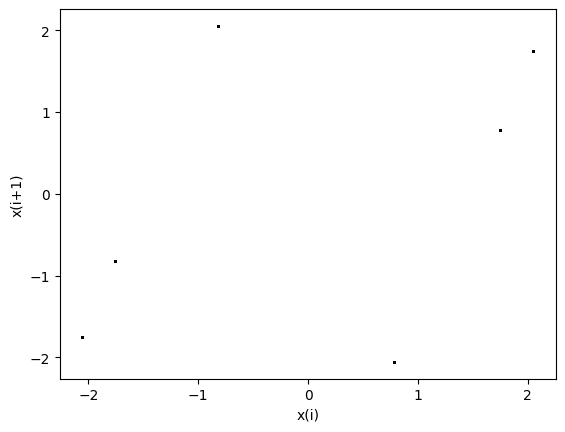
\includegraphics[width=\textwidth]{LateX images/sine q=-0.3/g7}
		\caption{Για $k=2.76$}
		\label{f:k120}
	\end{subfigure}
	\hfill		
	\caption{Διαγράμματα της τιμής \(x_i\) σε συνάρτηση με την τιμή \(x_{i+1}\) (α' μέρος).}
	\label{f:k246}
\end{figure}
\begin{figure}[ht]
	\centering
	\begin{subfigure}[b]{0.4\textwidth}
		\centering
		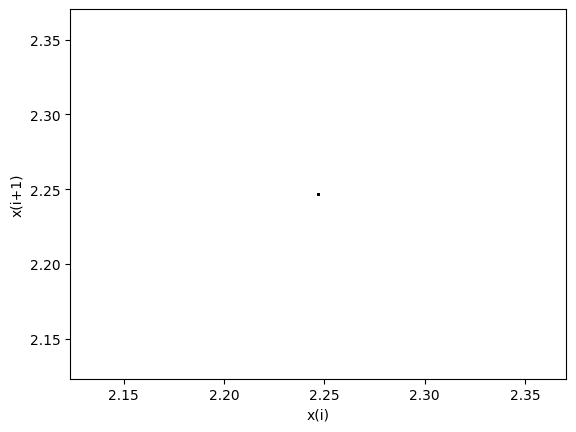
\includegraphics[width=\textwidth]{LateX images/sine q=-0.3/g8}
		\caption{Για $k=2.935$}
		\label{f:k121}
	\end{subfigure}
	\hfill
	\begin{subfigure}[b]{0.4\textwidth}
		\centering
		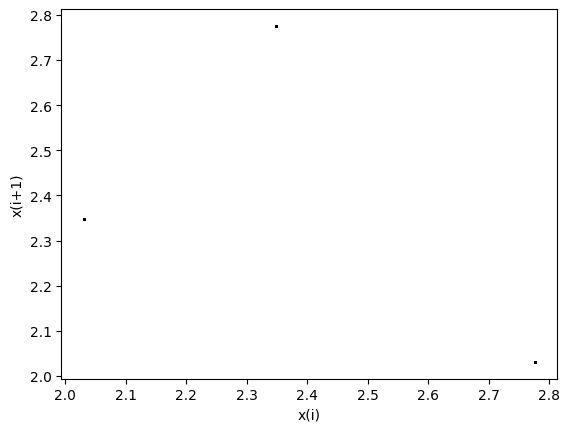
\includegraphics[width=\textwidth]{LateX images/sine q=-0.3/g9}
		\caption{Για $k=3.293$}
		\label{f:k122}
	\end{subfigure}
	\hfill
	\begin{subfigure}[b]{0.4\textwidth}
		\centering
		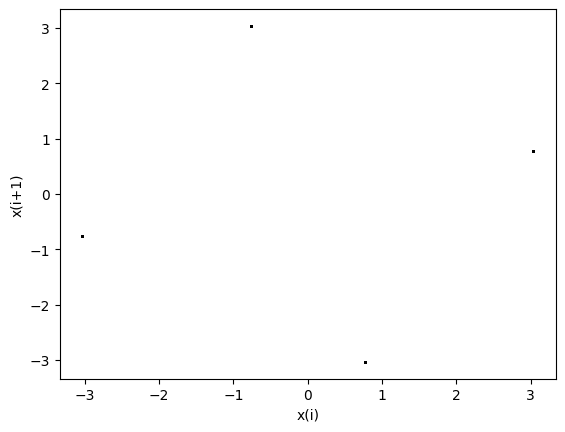
\includegraphics[width=\textwidth]{LateX images/sine q=-0.3/g10}
		\caption{Για $k=3.48$}
		\label{f:k123}
	\end{subfigure}
	\hfill
	\begin{subfigure}[b]{0.4\textwidth}
		\centering
		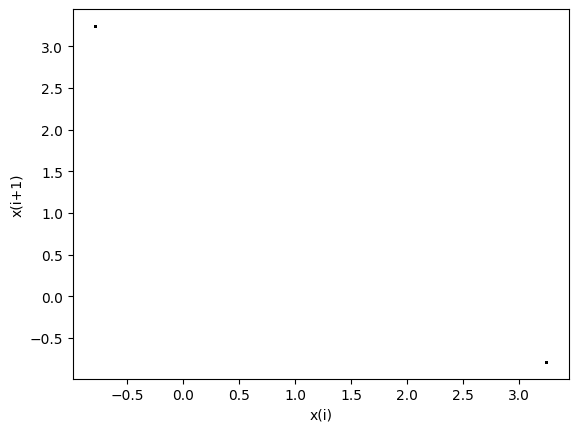
\includegraphics[width=\textwidth]{LateX images/sine q=-0.3/g11}
		\caption{Για $k=3.629$}
		\label{f:k124}
	\end{subfigure}
	\hfill
	\begin{subfigure}[b]{0.4\textwidth}
		\centering
		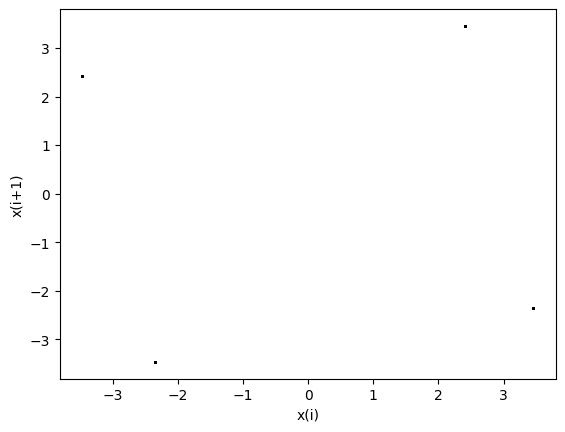
\includegraphics[width=\textwidth]{LateX images/sine q=-0.3/g12}
		\caption{Για $k=3.79$}
		\label{f:k125}
	\end{subfigure}
	\hfill
	\begin{subfigure}[b]{0.4\textwidth}
		\centering
		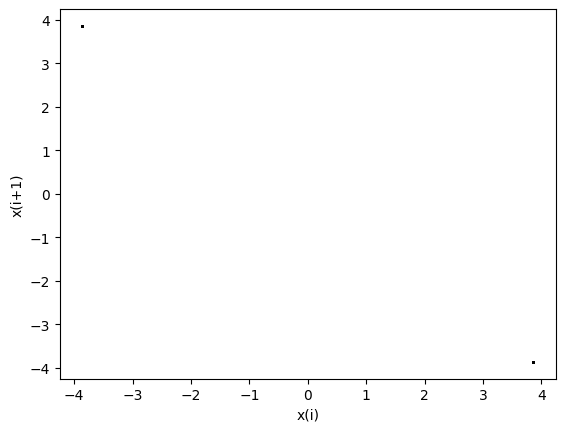
\includegraphics[width=\textwidth]{LateX images/sine q=-0.3/g13}
		\caption{Για $k=4.09$}
		\label{f:k126}
	\end{subfigure}
	\hfill
	\caption{Διαγράμματα της τιμής \(x_i\) σε συνάρτηση με την τιμή \(x_{i+1}\) (β' μέρος).}
	\label{f:k247}
\end{figure}

\clearpage 
\section{Για \emph{q} = -0.5}

Στο Σχ. \ref{f:48} παρατίθενται τα διαγράμματα διακλάδωσης του συστήματος \ref{f:x3}, ως προς την παράμετρο \emph{k}, για $b = 2$ , $q =-0.5$ και για διαφορετικές αρχικές συνθήκες, δηλαδή για διαφορετικό \(x_0\). Συγκρίνοντας το διάγραμμα του Σχ. \ref{f:g46} (\(x_0=0.1\)) με τα υπόλοιπα διαγράμματα διακλάδωσης των Σχ. \ref{f:g47} (\(x_0=0.5\)), \ref{f:g48} (\(x_0=1\)), παρατηρείται ότι για $q=-0.5$ εμφανίζεται το φαινόμενο της συνύπαρξης ελκυστών. Η συμπεριφορά του συστήματος για τις διάφορες περιπτώσεις επιβεβαιώνεται και από τα αντίστοιχα διαγράμματα Lyapunov των Σχ. \ref{f:g49}, \ref{f:g50}, \ref{f:g51}, όπως και απο το διάγραμμα διακλάδωσης του Σχ. \ref{f:g54}, όπου η κάθε αρχική συνθήκη εμφανίζεται με διαφορετικό χρώμα.

Στον Πίνακα \ref{tab:abc11} φαίνεται η πορεία του συστήματος και για ποιες τιμές της παραμέτρου \emph{k} το σύστημα εμφανίζει περιοδική ή χαοτική συμπεριφορά, σύμφωνα με το διάγραμμα διακλάδωσης του Σχ. \ref{f:g46}. Οι τιμές αυτές αντιστοιχούν στα σχήματα των διαγραμμάτων της τιμής \(x_i\) σε συνάρτηση με την τιμή \(x_{i+1}\). Από τα παραγόμενα Σχ. \ref{f:g58} προκύπτει αριθμός σημείων αντίστοιχος με την περίοδο του συστήματος.

Επίσης παρατηρείται η εσωτερική κρίση ελκυστών για διάφορες τιμές του \emph{k} (1.773, 1.8, 1.831, 1.93, 2.03, 2.141, 2.2, 2.38,
2.88, 2.99, 3.04, 3.2, 3.35, 3.4, 3.44, 3.62, 3.93), όπως και το φαινόμενο της υστέρησης το οποίο φαίνεται στο διάγραμμα διακλάδωσης του Σχ. \ref{f:g46} στην μεταπήδηση του συστήματος από χαοτική συμπεριφορά σε \emph{περίοδο-1}, και \emph{περίοδο - 2}. Οι αντίστοιχες τιμές του \emph{k} για αυτά τα σημεία του διαγράμματος υπάρχουν στο Πίνακα \ref{tab:abc11}.

Επιπλέον παρατηρούμε στα διαγράμματα των Σχ. \ref{f:g52}, \ref{f:g53}, \ref{f:g533} το φαινόμενο της αντιμονοτονικότητας. Συγκεκριμένα στο διάγραμμα του Σχ. \ref{f:g52} εμφανίζεται μία χαοτική φυσαλίδα (το σύστημα εισέρχεται στο χάος με διπλασιασμό της περιόδου και στην συνέχεια εξέρχεται από αυτό με αντίστροφο διπλασιασμό της περιόδου), για $k=3.84$, της οποίας η εξέλιξη φαίνεται στα υπόλοιπα δύο διαγράμματα των. Σχ. \ref{f:g53}, \ref{f:g533}, όπου για διαφορετικές αρχικές συνθήκες $x_0$ διακρίνεται καλύτερα. Ακόμη στο διάγραμμα του Σχ. \ref{f:g48} το φαινόμενο εμφανίζεται άλλη μία φορά για $3.95<k<4.05$.
Μεταξύ αυτών των χαοτικών φυσαλίδων παρατηρούμε και τις δύο περιπτώσεις του φαινομένου δηλαδή τον ορθό και τον ανάστροφο διπλασιασμό της περιόδου.%%%βάλε λαμπελ για την θεωρία%% 
Στα Σχ. \ref{f:g54}, \ref{f:g55}, \ref{f:g56} παρατηρείται ότι για $k=3.206$ εμφανίζεται ένας διπλασιασμός (\emph{περίοδος - 4}) ο οποίος καταστρέφεται για $k=3.23$, οπότε εδώ παρατηρούμε το φαινόμενο της αντιμονοτονικότητας δηλαδή έχουμε μία ανάστροφη ακολουθία διπλασιασμού της περιόδου για $k=3.23$. 

Τέλος, στο σχήμα \ref{f:g23} παρατίθεται το διάγραμμα των εκθετών Lyapunov για τιμές του \emph{k} στο ίδιο διάστημα τιμών $[0, 4.2]$. Οι τιμές του Πίνακα \ref{tab:abc11} που έχουν περιοδική συμπεριφορά αντιστοιχούν σε τιμές του διαγράμματος του Σχ. \ref{f:g49}, όπου ο εκθέτης Lyapunov είναι συνεχώς αρνητικός, γεγονός που επιβεβαιώνει την συμπεριφορά τους. Ενώ για τις υπόλοιπες τιμές ο θετικός εκθέτης Lyapunov υποστηρίζει την χαοτική τους συμπεριφορά, όπως έγινε φανερό και από το διάγραμμα διακλάδωσης.





\begin{table}[ht]
	\centering
	\caption{ Συμπεριφορά του υπό μελέτη συστήματος για διάφορες τιμές του \emph{k}, για $q=-0.5$ }
	\label{tab:abc11}
	\begin{tabular}{l | l}
		Παράμετρος k & Συμπεριφορά \\
		\hline
		0.25 &  Περίοδος -  1 \\
		1 &  Περίοδος -  2 \\
		1.7& Περίοδος -  4 \\
		1.748& Περίοδος -  8 \\
		1.75 & Xάος \\
		1.773& Περίοδος - 6 \\
		1.774& Περίοδος - 12\\
		1.775& Χάος \\
		1.8& Περίοδος - 10 \\
		1.806 &  Χάος \\
		1.831 &  Περίοδος -  6 \\
		1.84 &  Χάος \\
		1.93 & Περίοδος - 6\\
		1.935 &Χάος \\
		2.03 &  Περίοδος -  4\\
		2.06 &Χάος \\
		2.141 & Περίοδος -  6\\
		2.144& Χάος\\
		2.2& Περίοδος - 6\\
		2.25& Χάος\\
		2.38 & Περίοδος -  1\\
		2.69 & Περίοδος -  2\\
		2.81 & Περίοδος -  4\\
		2.83 & Περίοδος -  8\\
		2.84 & Χάος\\
		2.88& Περίοδος -  3\\
		2.89 & Χάος\\
		2.99 &  Περίοδος -  6\\
		3 &  Περίοδος - 12\\
		3.01 &  Χάος\\
		3.04 & Περίοδος - 4\\
		3.08 & Χάος\\
		3.2 & Περίοδος -2\\
		3.206 & Περίοδος -  4\\
		3.23 & Περίοδος -  2\\
		3.24 & Χάος\\
		3.35 & Περίοδος -  4\\
		3.36 & Χάος\\
		3.4 & Περίοδος -  4\\
		3.41 & Χάος\\
		3.44 & Περίοδος -  4\\
		3.45 & Χάος\\
		3.62 & Περίοδος -  2\\
		3.8 & Περίοδος -  4\\
		3.84 & Χάος\\
		3.94 & Περίοδος -  8\\
		3.95 & Περίοδος -  4\\
		3.96 & Περίοδος -  8\\
		3.97 & Περίοδος -  16\\
		3.98 & Χάος\\
		4 & Περίοδος -  6\\
		4.05&Περίοδος - 4\\
		4.07 & Χάος\\
		
	\end{tabular}
	
\end{table}


\begin{figure}[ht]
	\centering
	\begin{subfigure}[b]{0.8\textwidth}
		\centering
		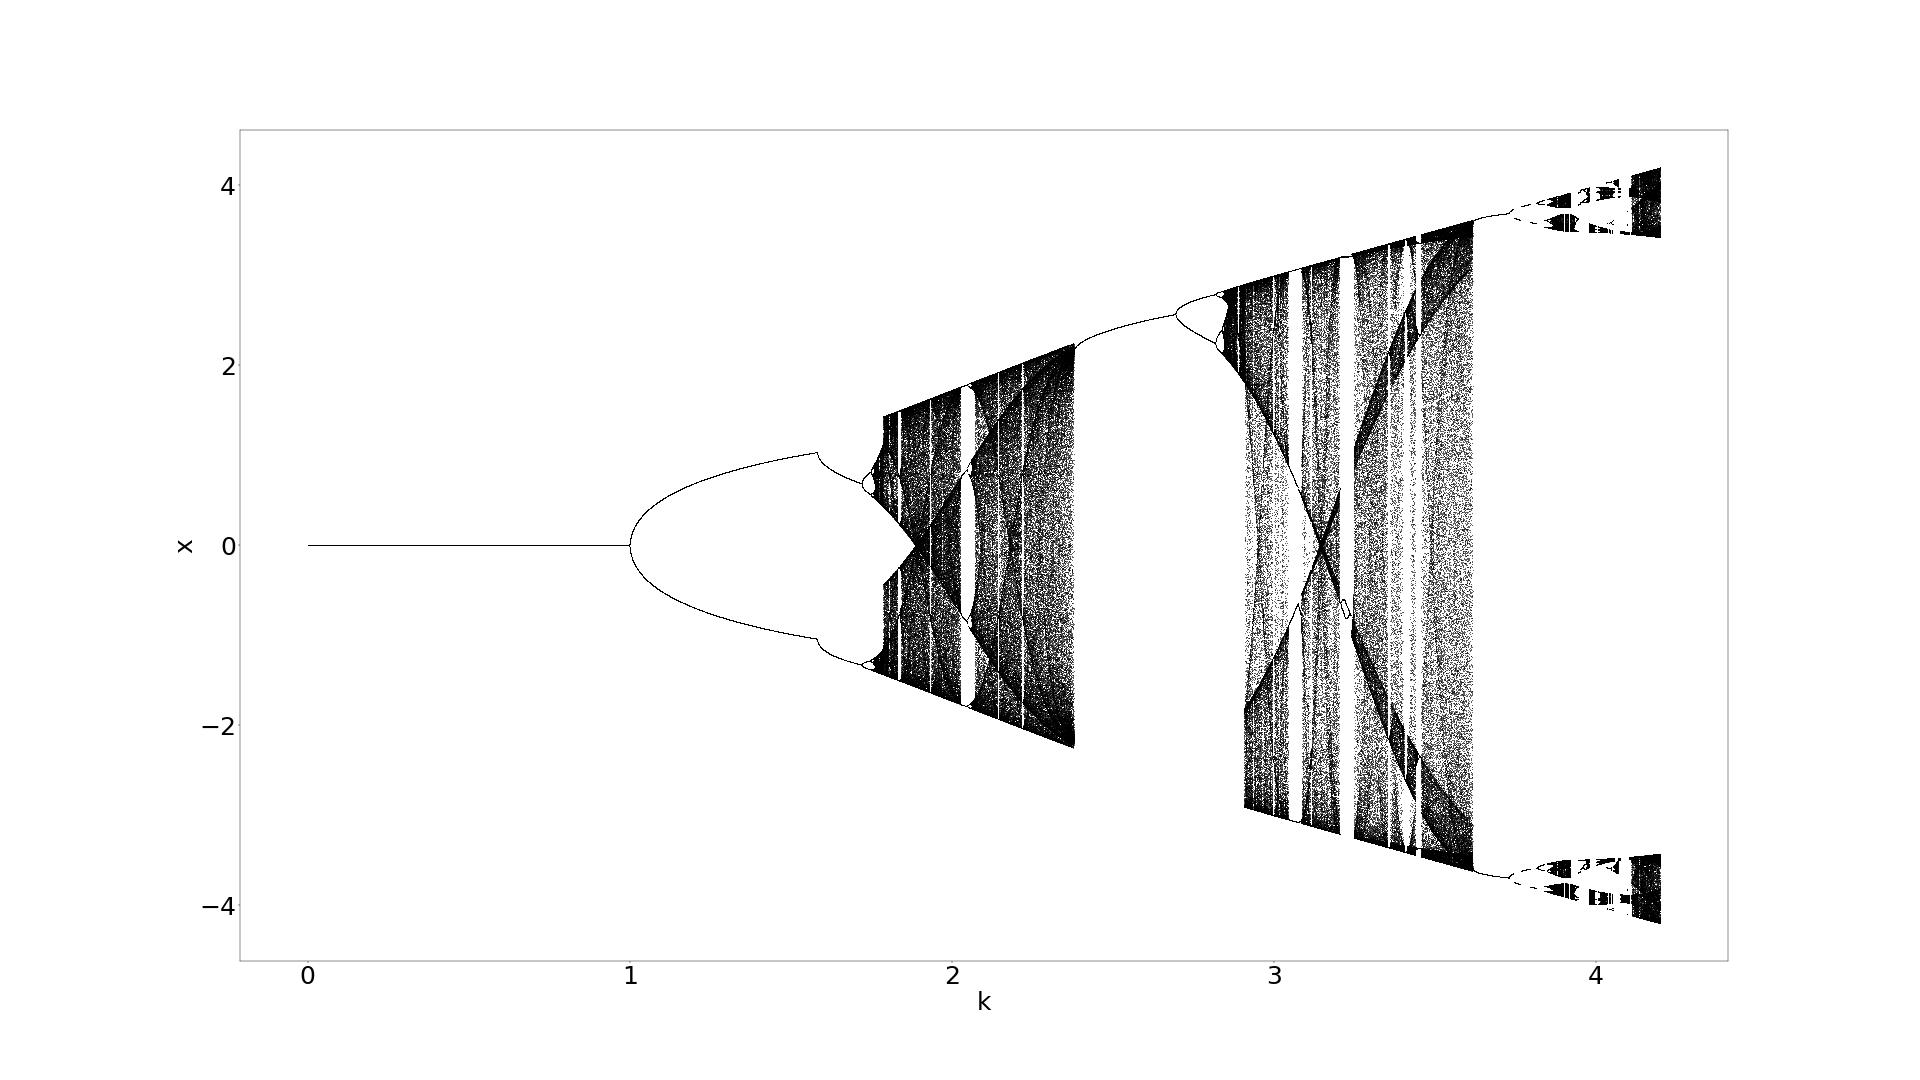
\includegraphics[width=\textwidth]{LateX images/sine q=-0.5/g4}
		\caption{\(x_0=0.1\)}
		\label{f:g46}
	\end{subfigure}
	\hfill
	\begin{subfigure}[b]{0.8\textwidth}
		\centering
		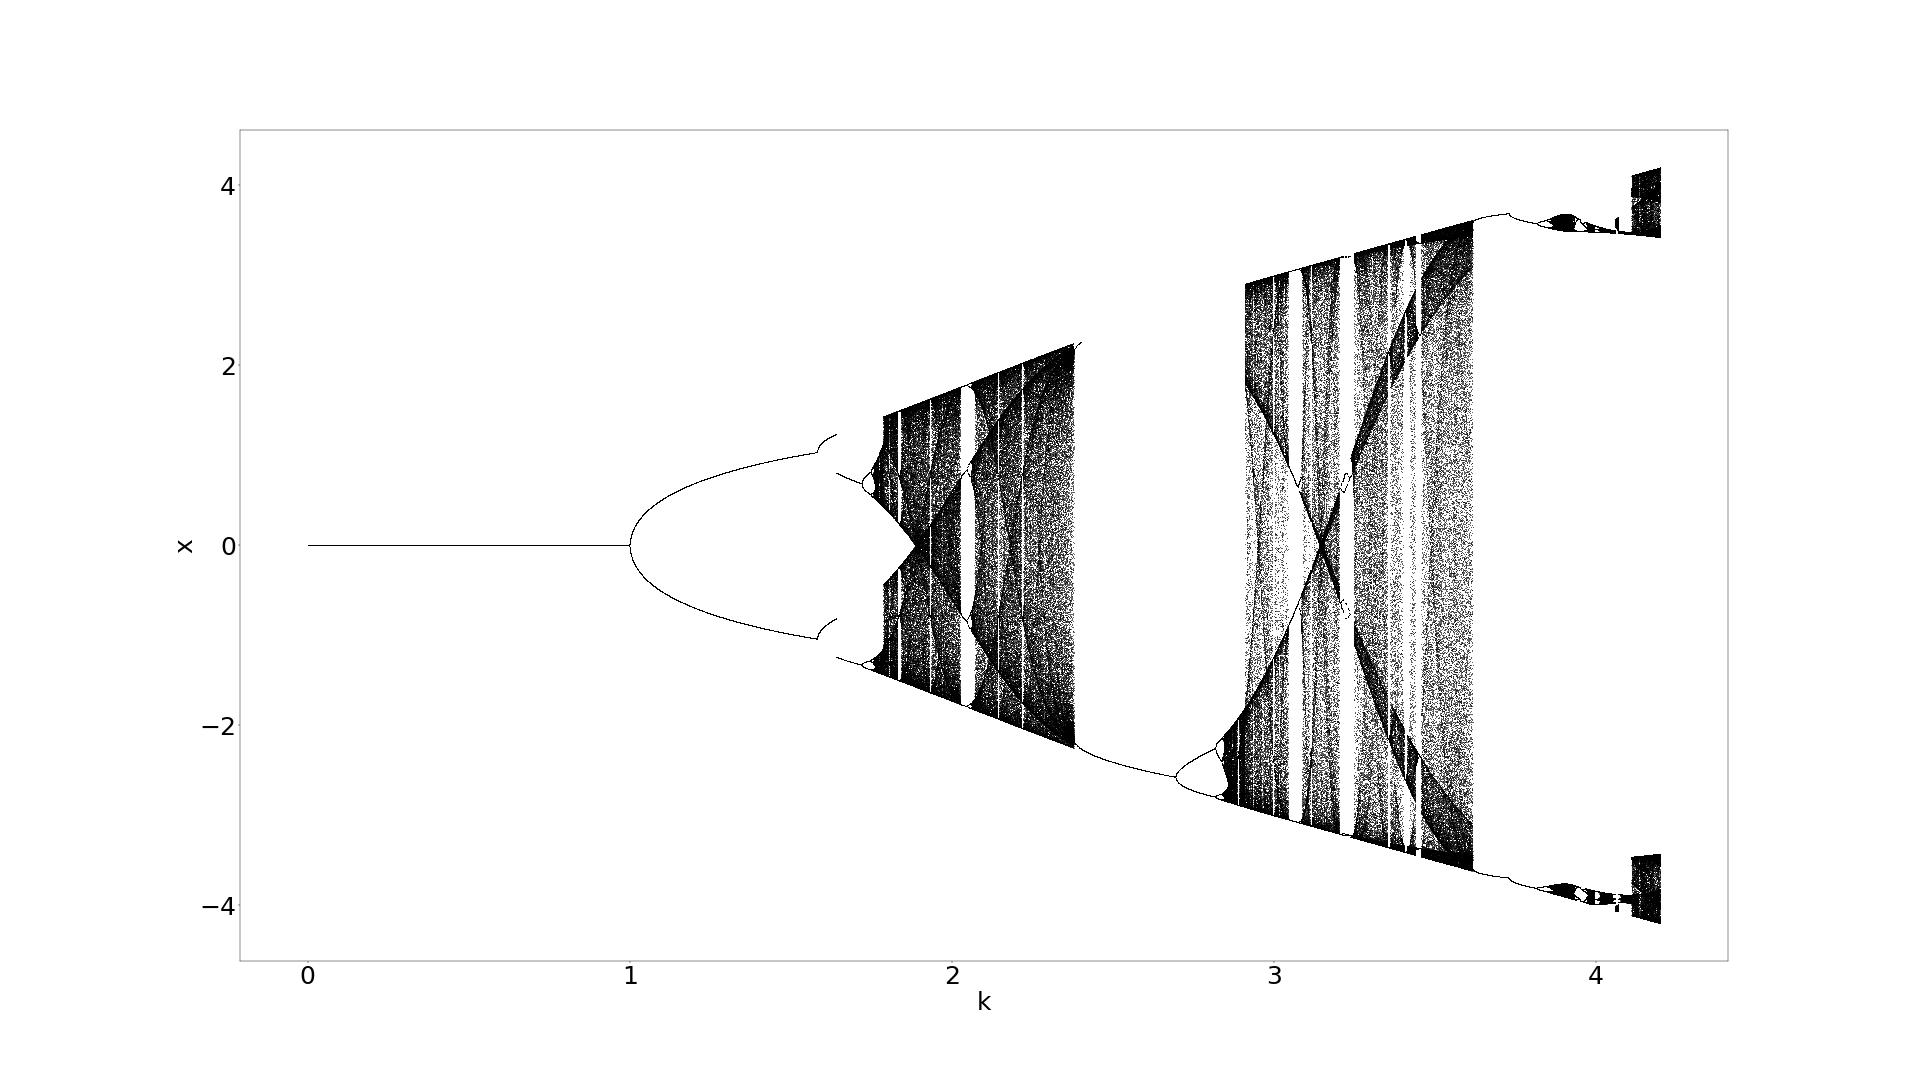
\includegraphics[width=\textwidth]{LateX images/sine q=-0.5/g5}
		\caption{\(x_0=0.5\)}
		\label{f:g47}
	\end{subfigure}
	\hfill
	\begin{subfigure}[b]{0.8\textwidth}
		\centering
		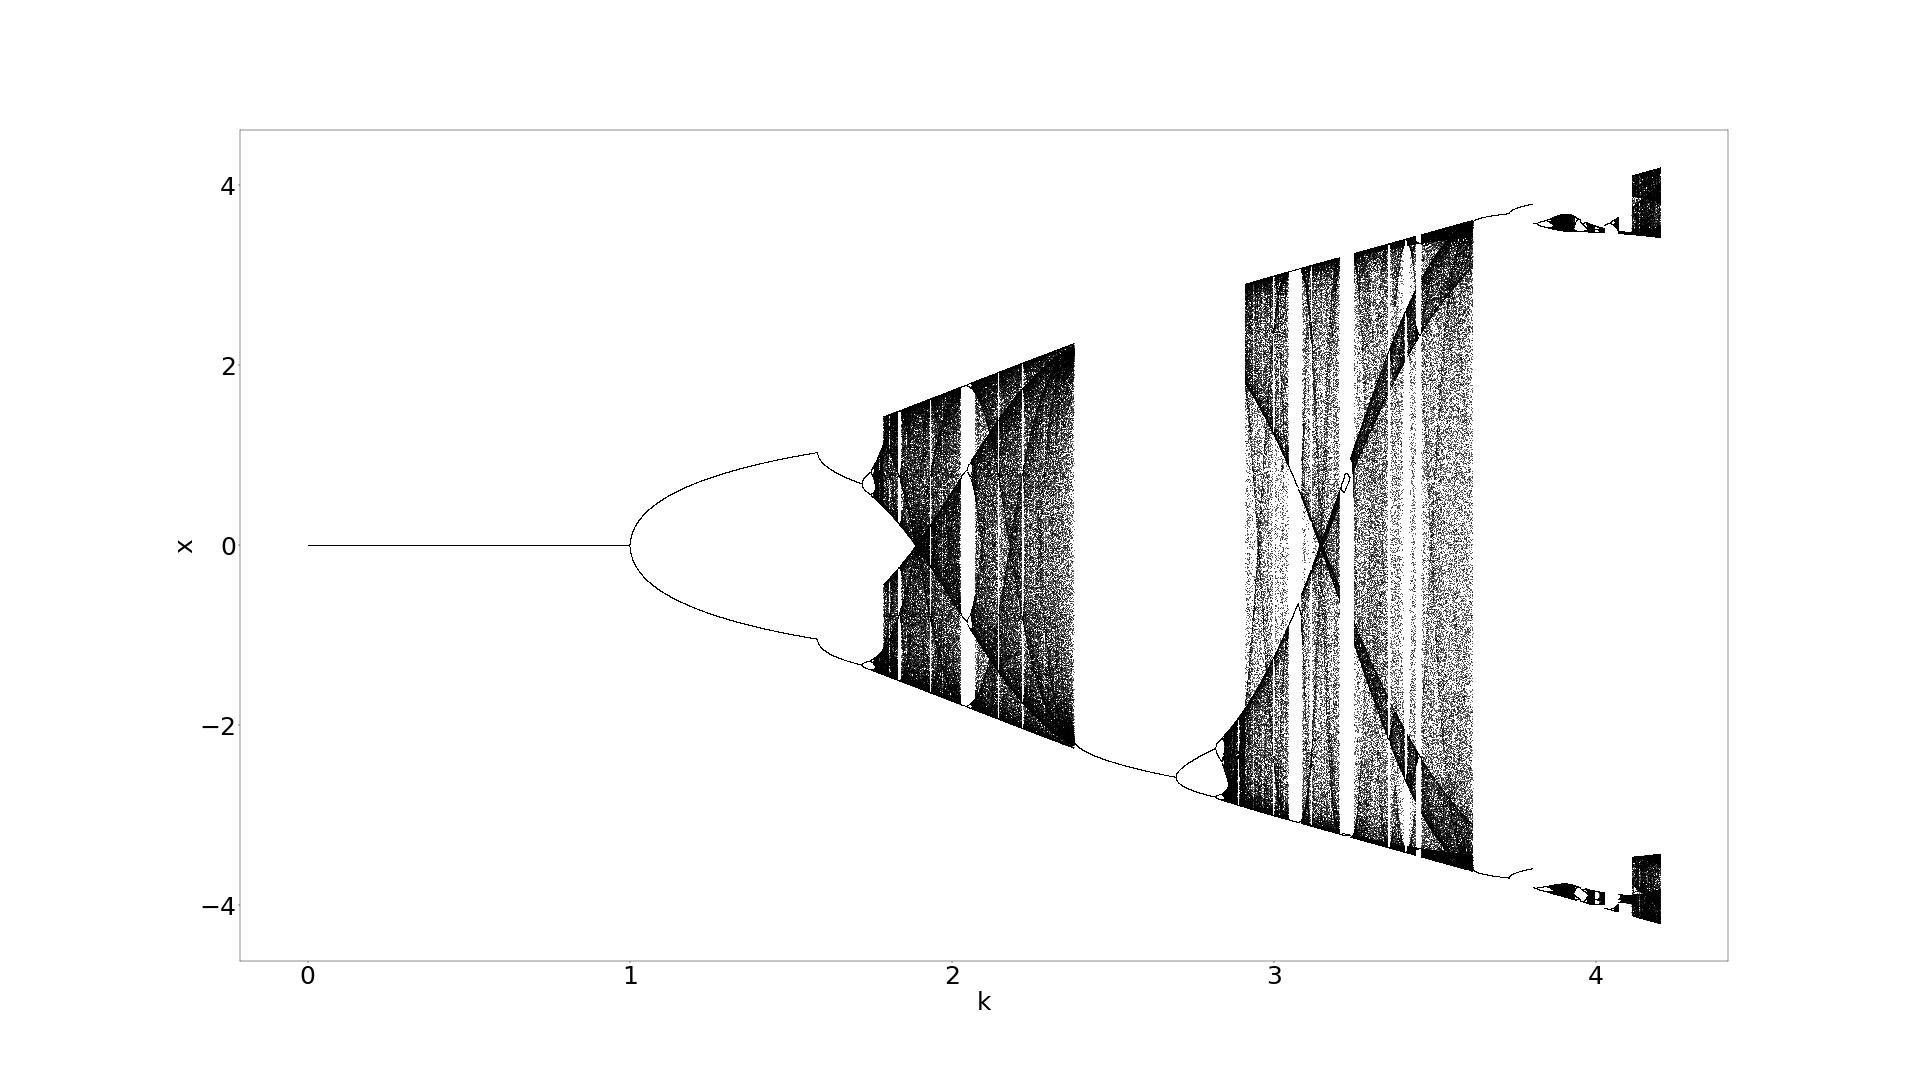
\includegraphics[width=\textwidth]{LateX images/sine q=-0.5/g6}
		\caption{\(x_0=1\)}
		\label{f:g48}
	\end{subfigure}
	\caption{ Διαγράμματα διακλάδωσης, για $b = 2$, $q=-0.5$}
	\label{f:48}
\end{figure}

\begin{figure}[ht]
	\centering
	
	\begin{subfigure}[b]{0.8\textwidth}
		\centering
		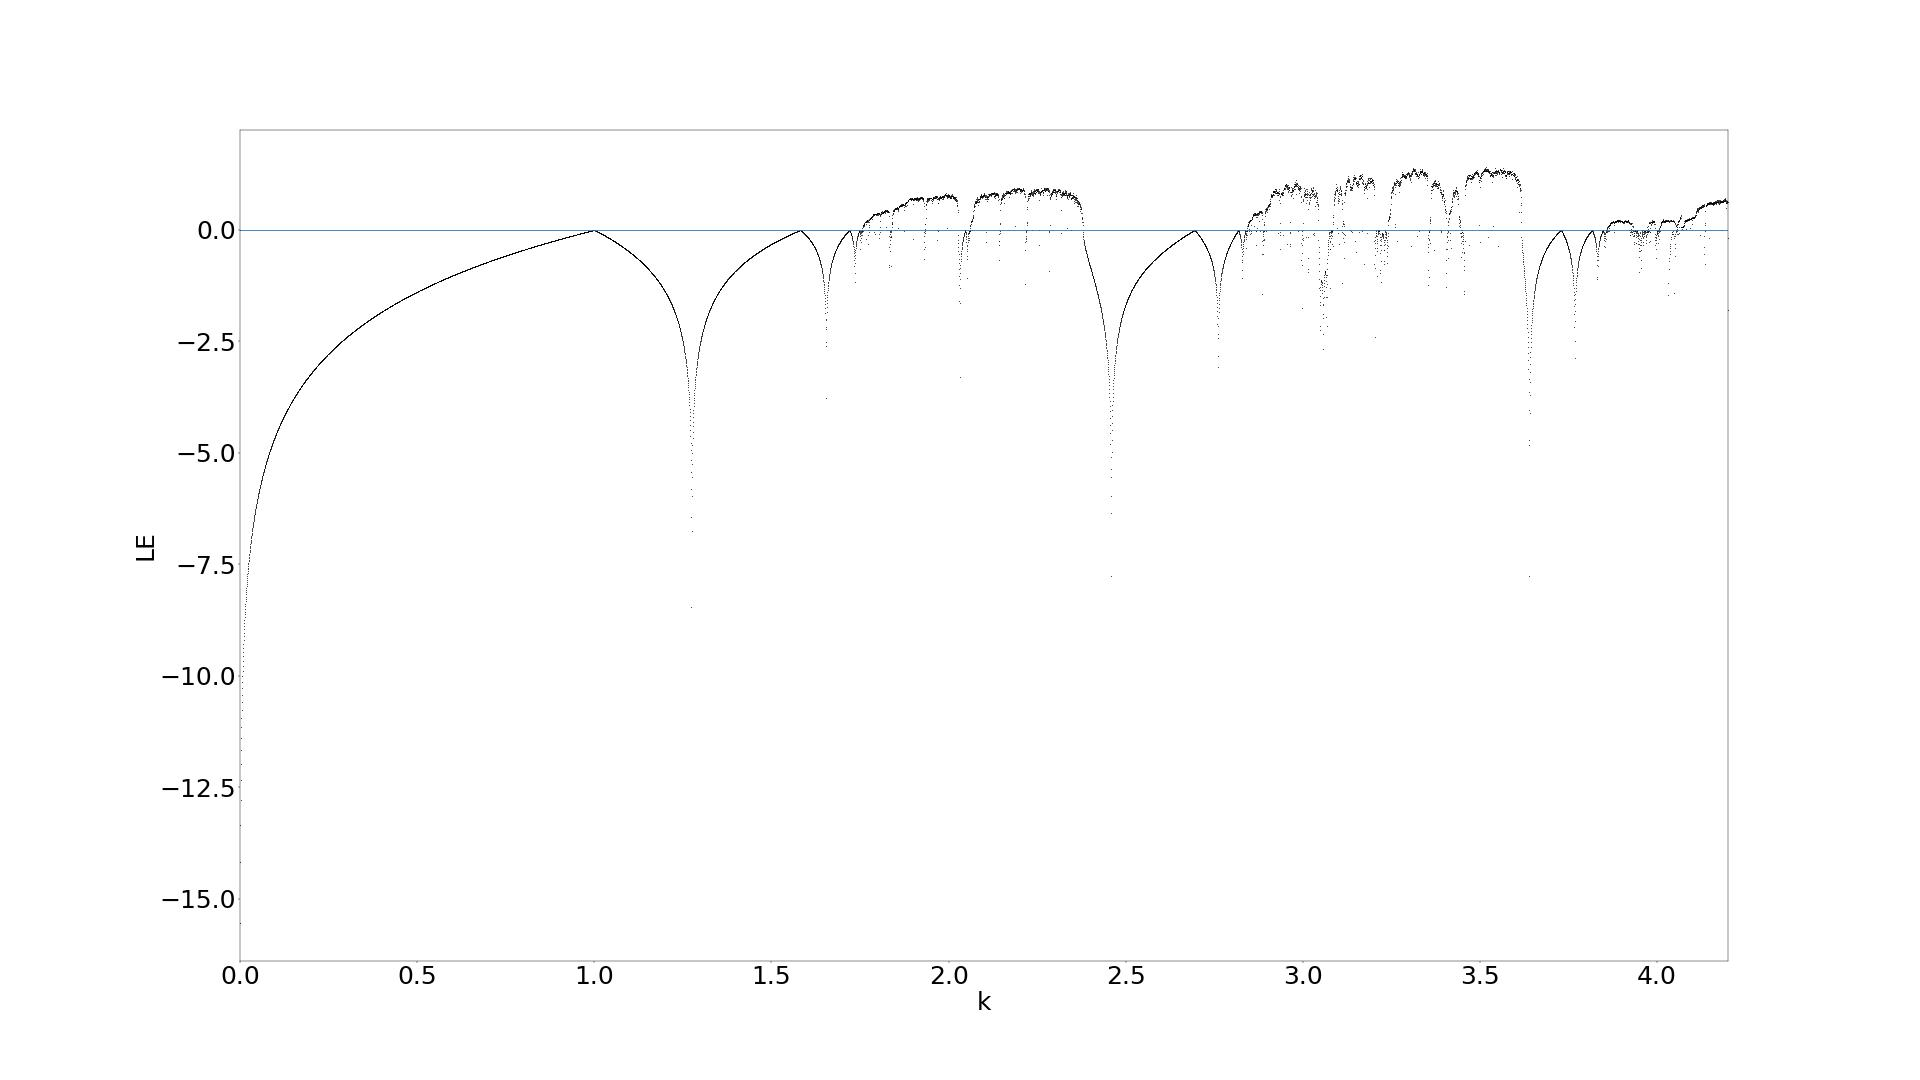
\includegraphics[width=\textwidth]{LateX images/sine q=-0.5/g8}
		\caption{Για \(x_0=0.1\)}
		\label{f:g49}
	\end{subfigure}
	\hfill
	\begin{subfigure}[b]{0.8\textwidth}
		\centering
		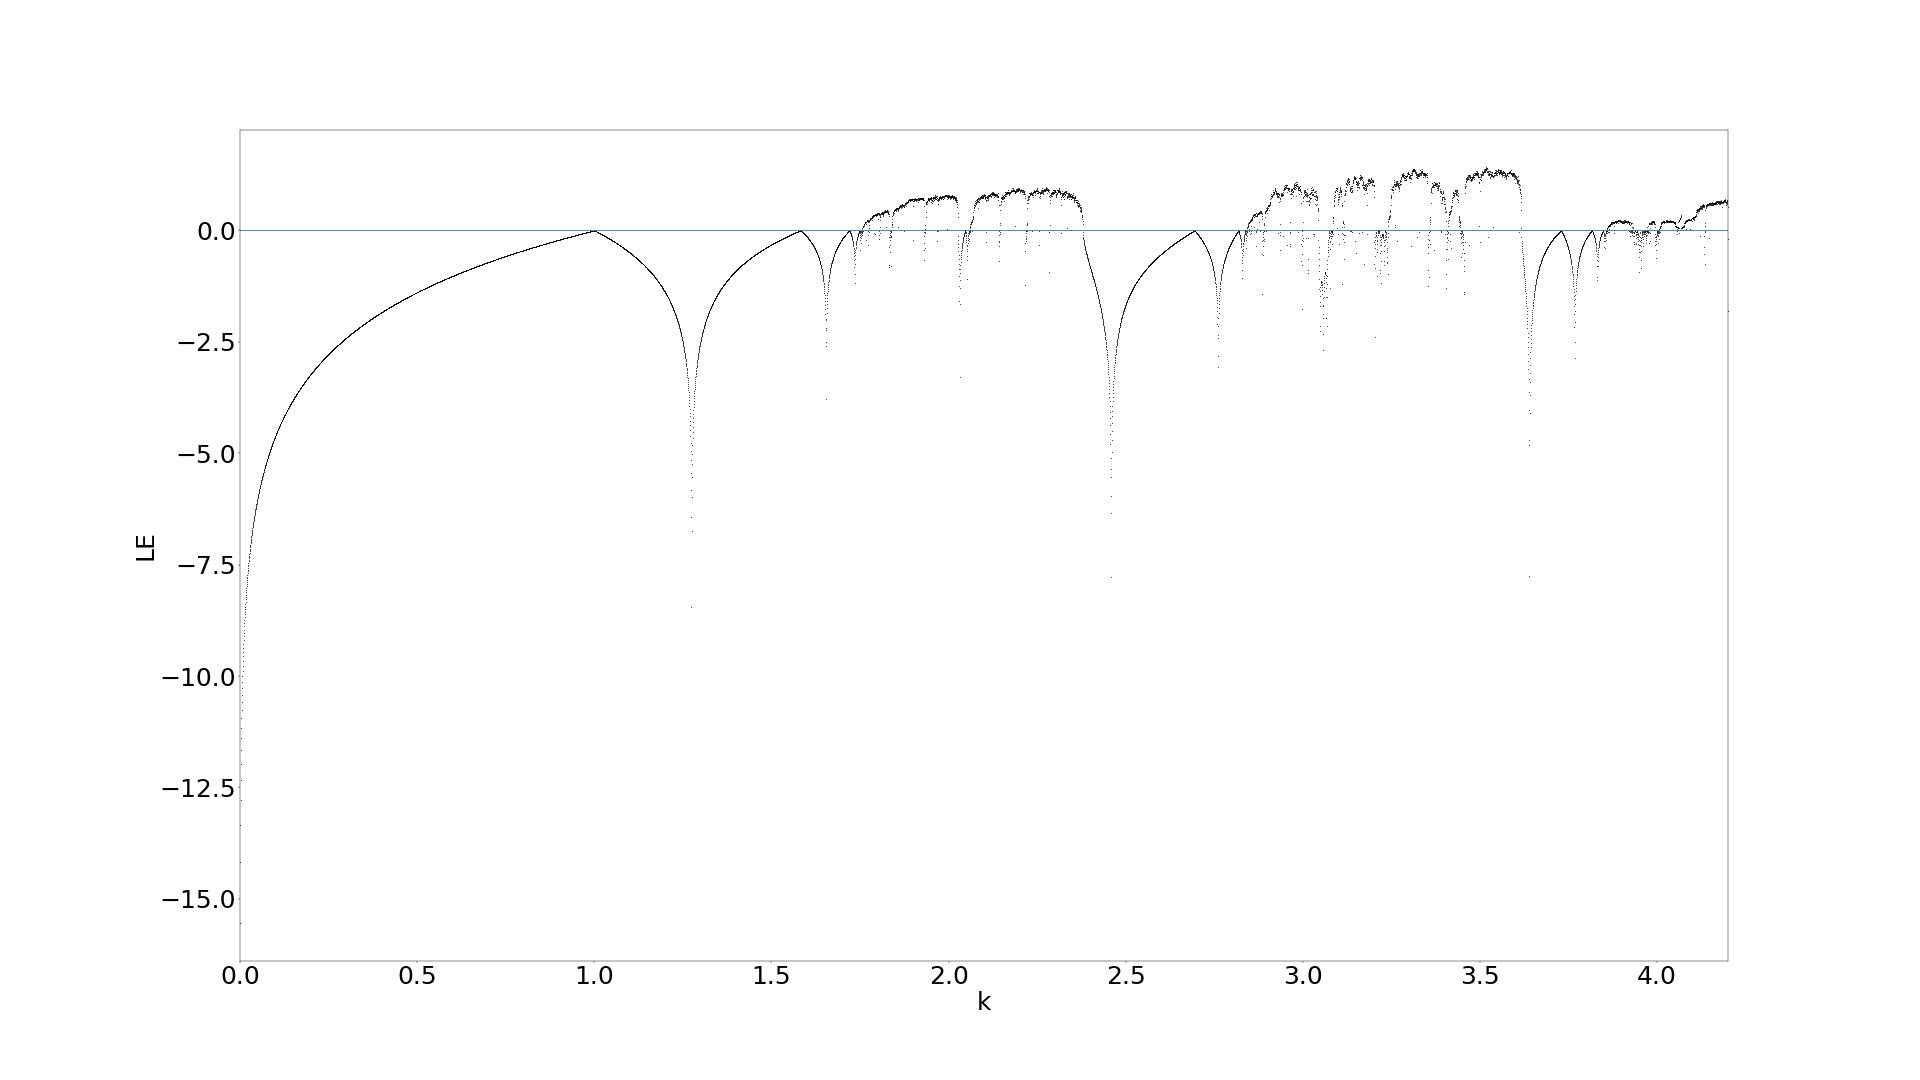
\includegraphics[width=\textwidth]{LateX images/sine q=-0.5/g9}
		\caption{Για \(x_0=0.5\)}
		\label{f:g50}
	\end{subfigure}
	\hfill
	\begin{subfigure}[b]{0.8\textwidth}
		\centering
		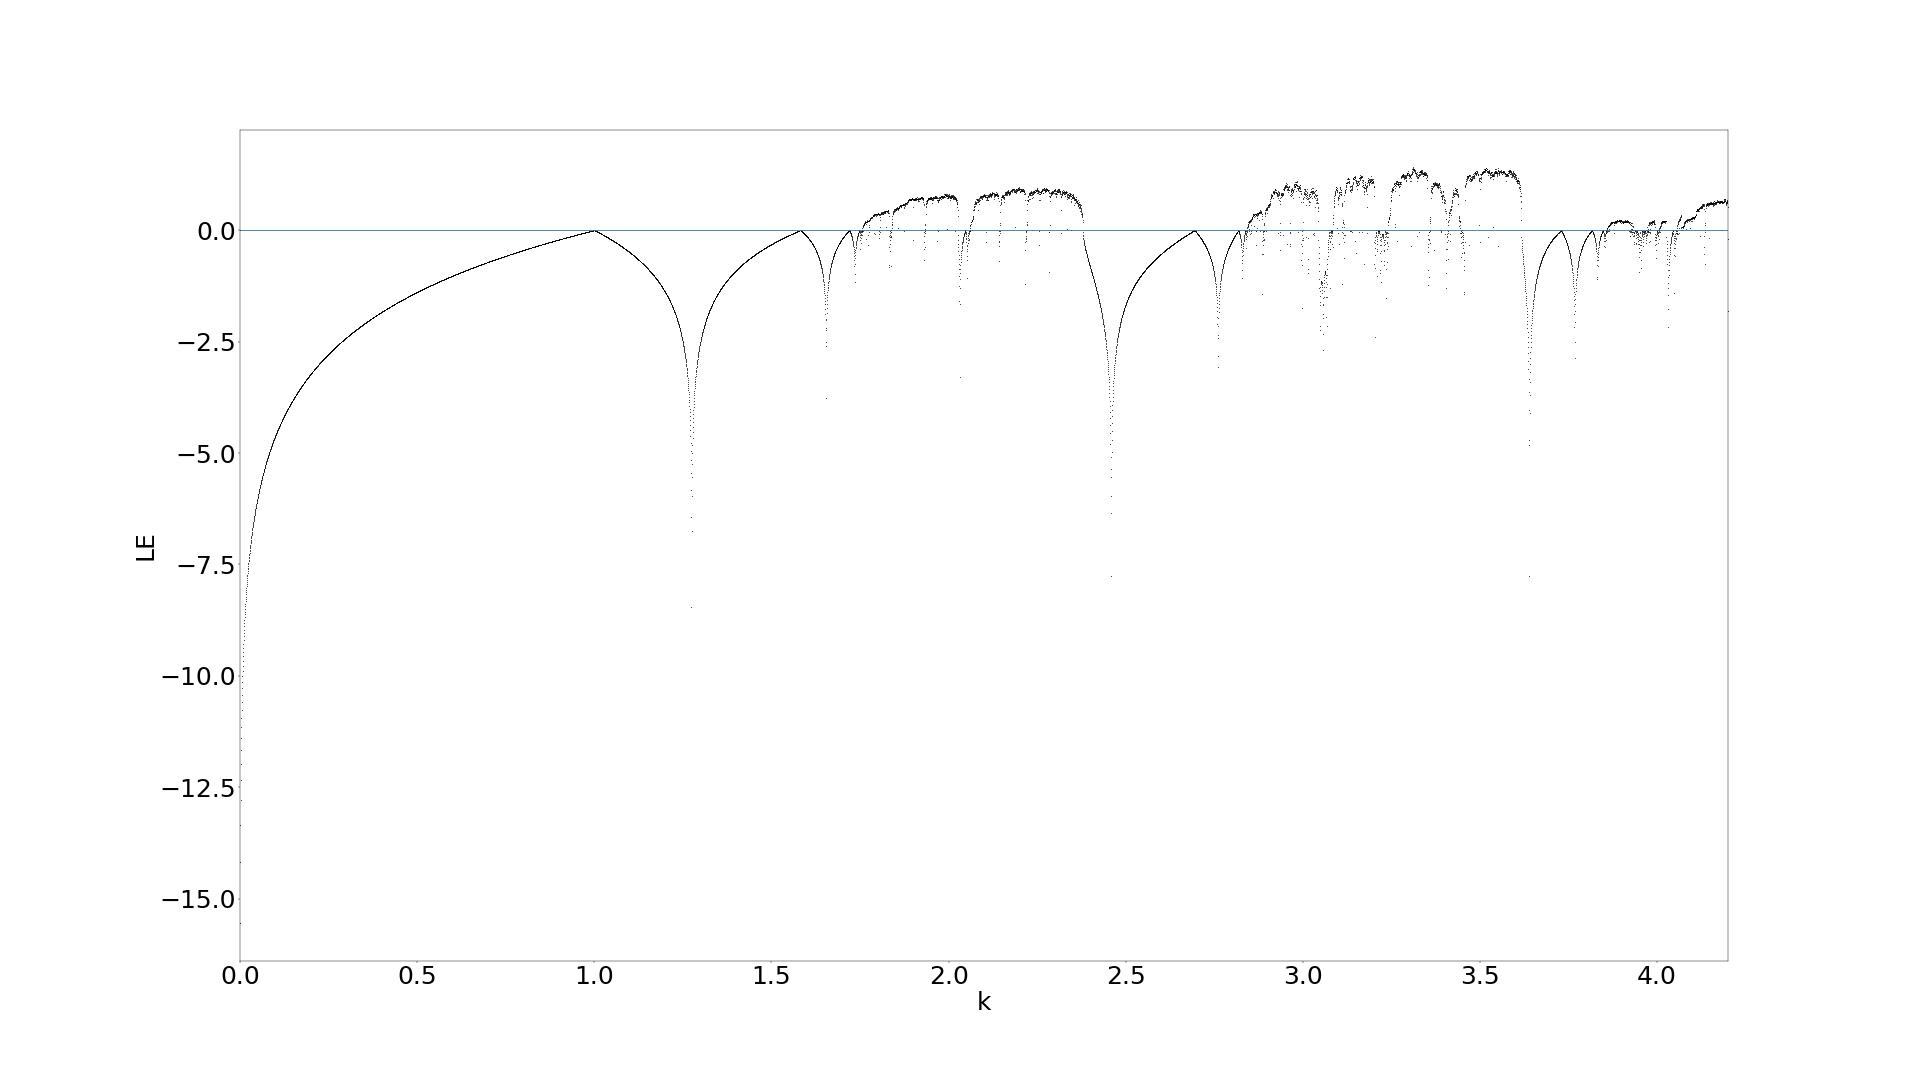
\includegraphics[width=\textwidth]{LateX images/sine q=-0.5/g10}
		\caption{Για \(x_0=1\)}
		\label{f:g51}
	\end{subfigure}
	\hfill
	\caption{ Διαγράμματα των εκθετών Lyapunov σε συνάρτηση με την παράμετρο \emph{k}, για $b = 2$, $q=-0.5$.}
	\label{f:g236}
\end{figure}


\begin{figure}[ht]
	\centering
	
	\begin{subfigure}[b]{0.8\textwidth}
		\centering
		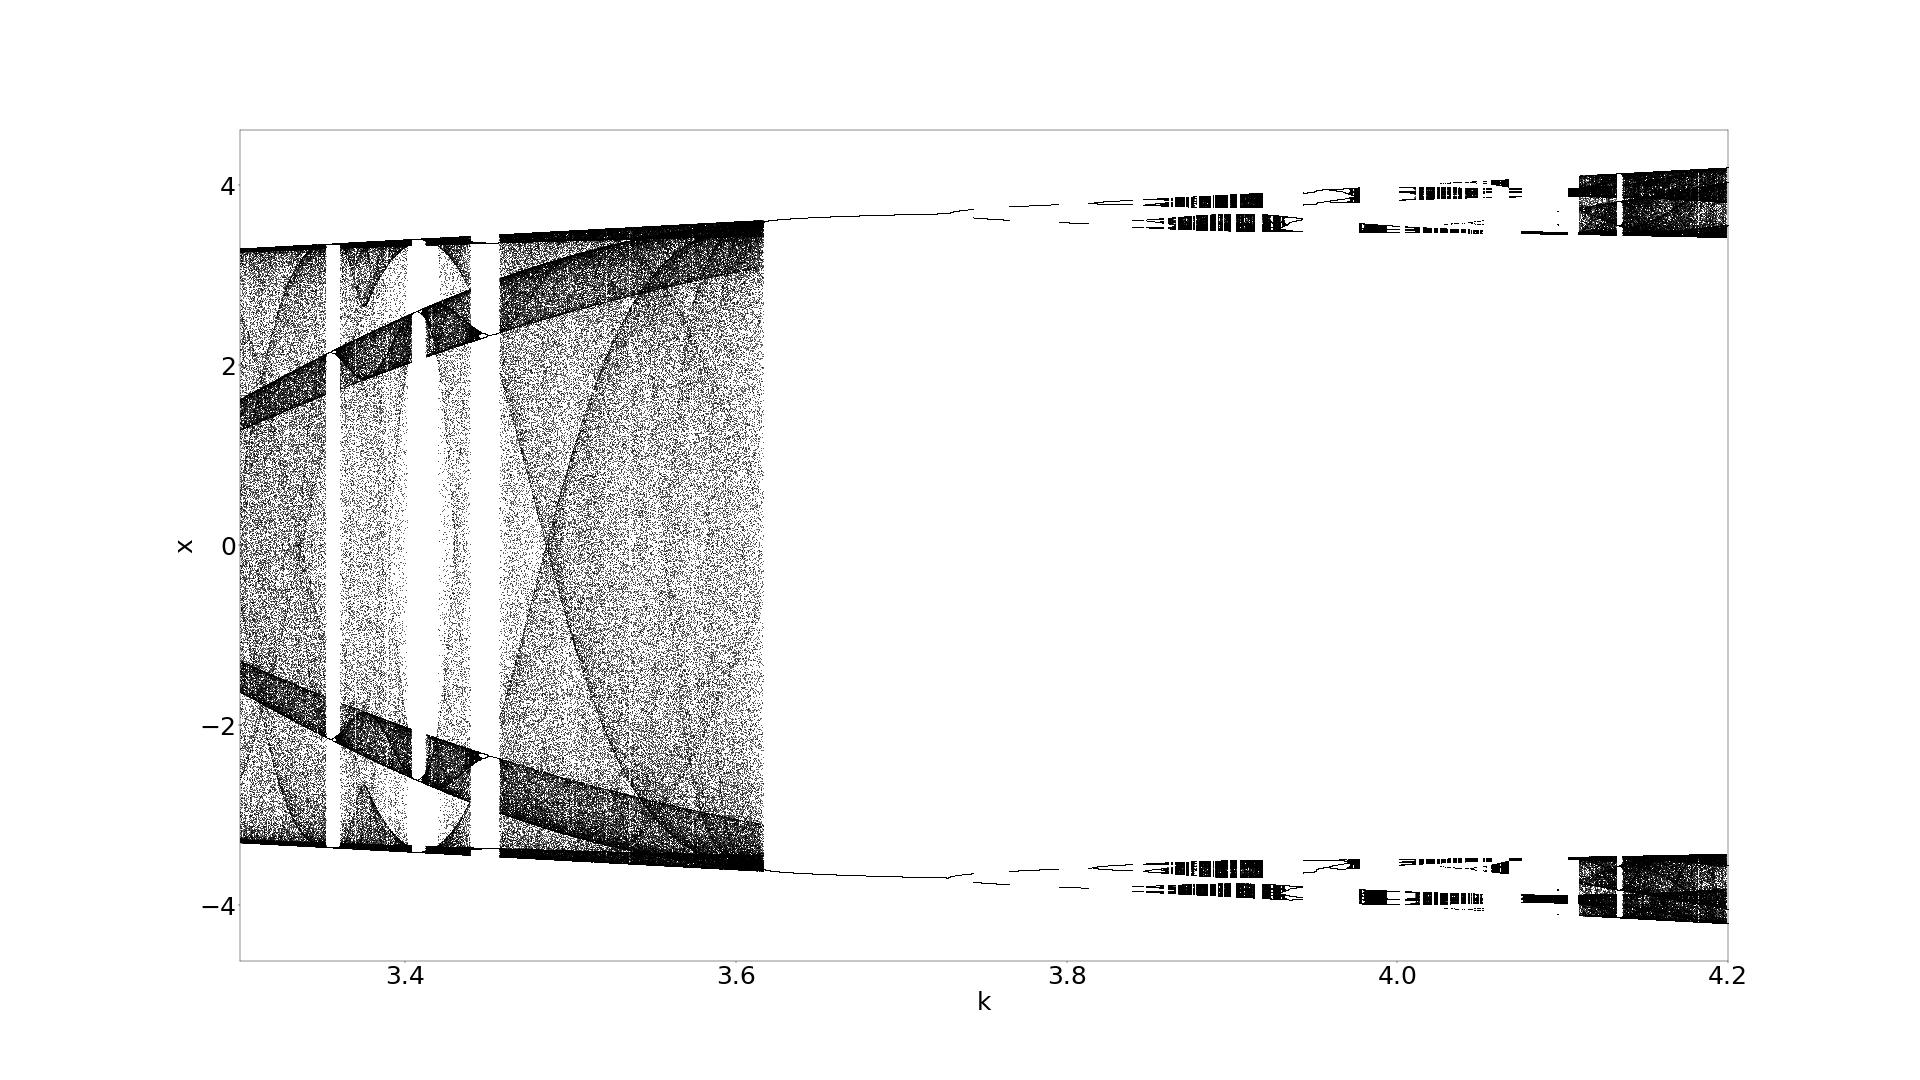
\includegraphics[width=\textwidth]{LateX images/sine q=-0.5/g3}
		\caption{$x_0=0.1$}
		\label{f:g52}
	\end{subfigure}
	\hfill
	\begin{subfigure}[b]{0.8\textwidth}
		\centering
		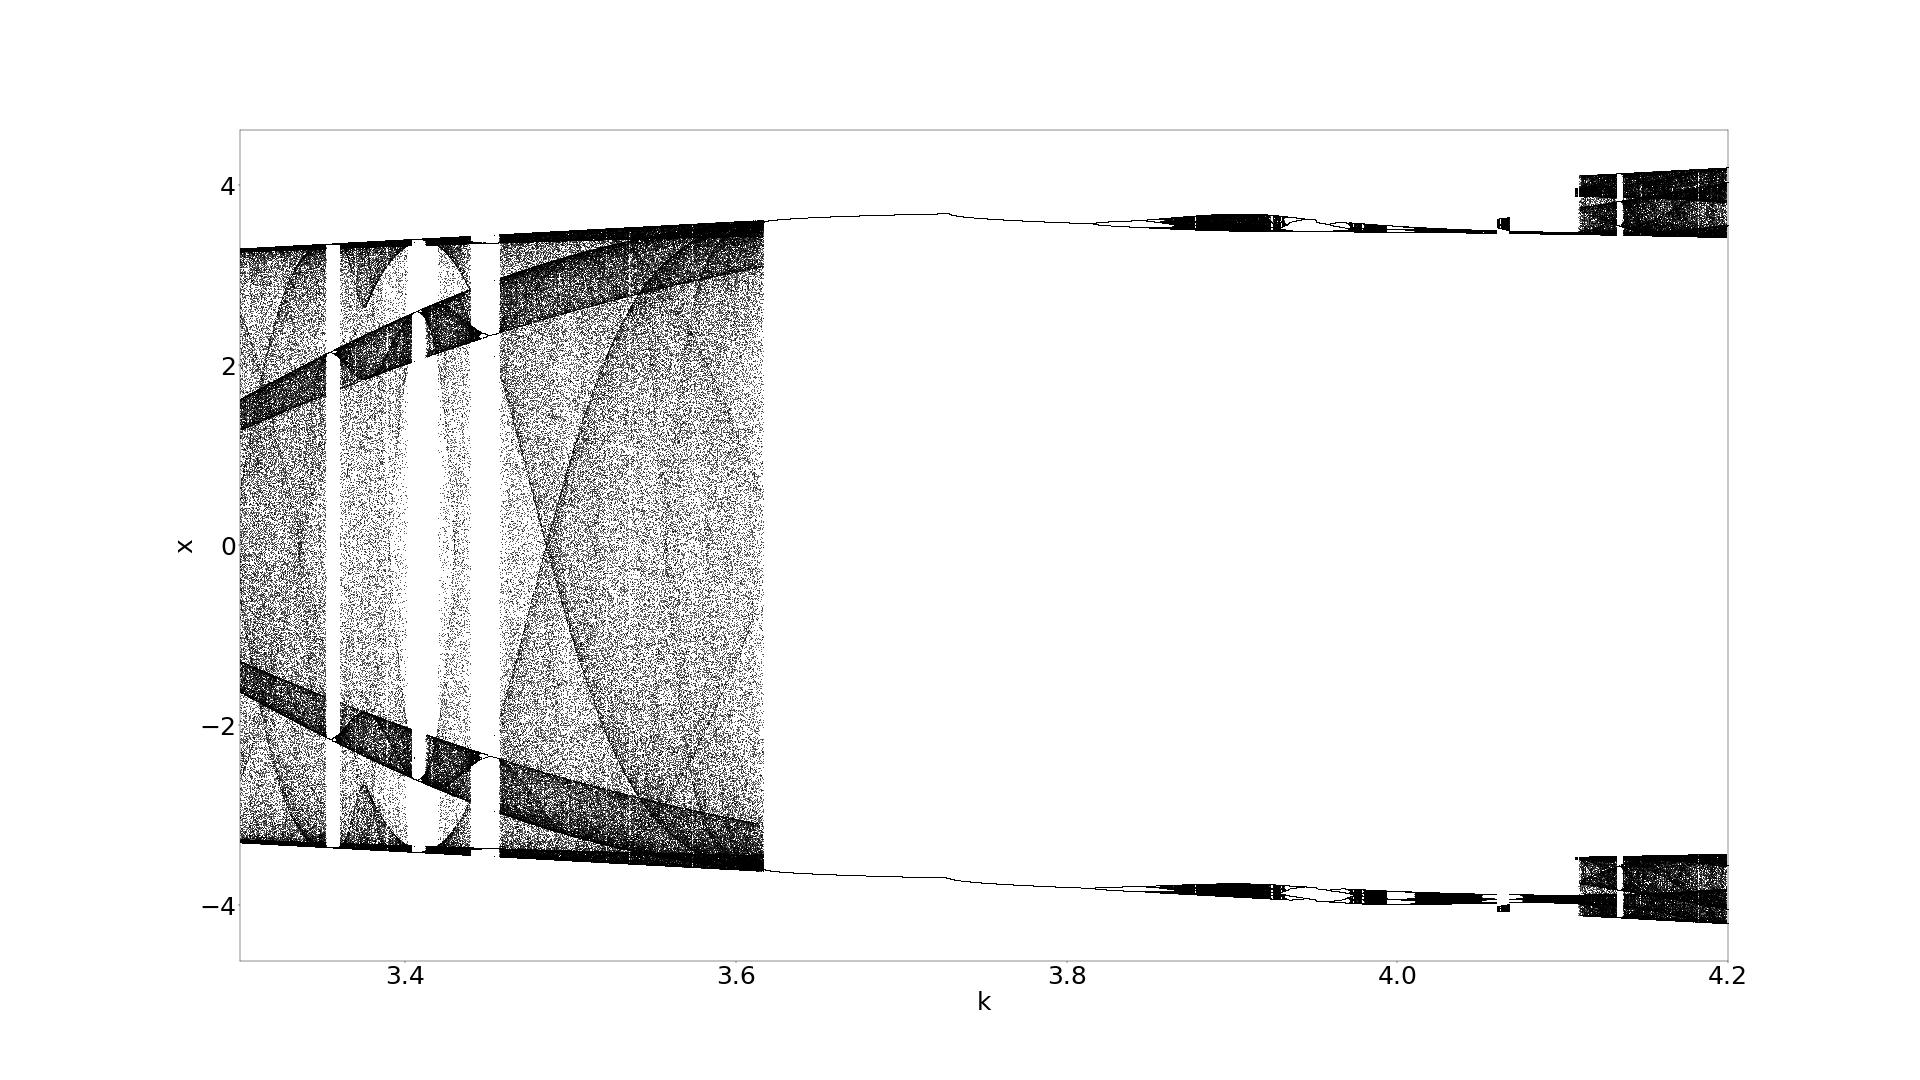
\includegraphics[width=\textwidth]{LateX images/sine q=-0.5/g7}
		\caption{$x_0=0.5$}
		\label{f:g53}
	\end{subfigure}
	\begin{subfigure}[b]{0.8\textwidth}
		\centering
		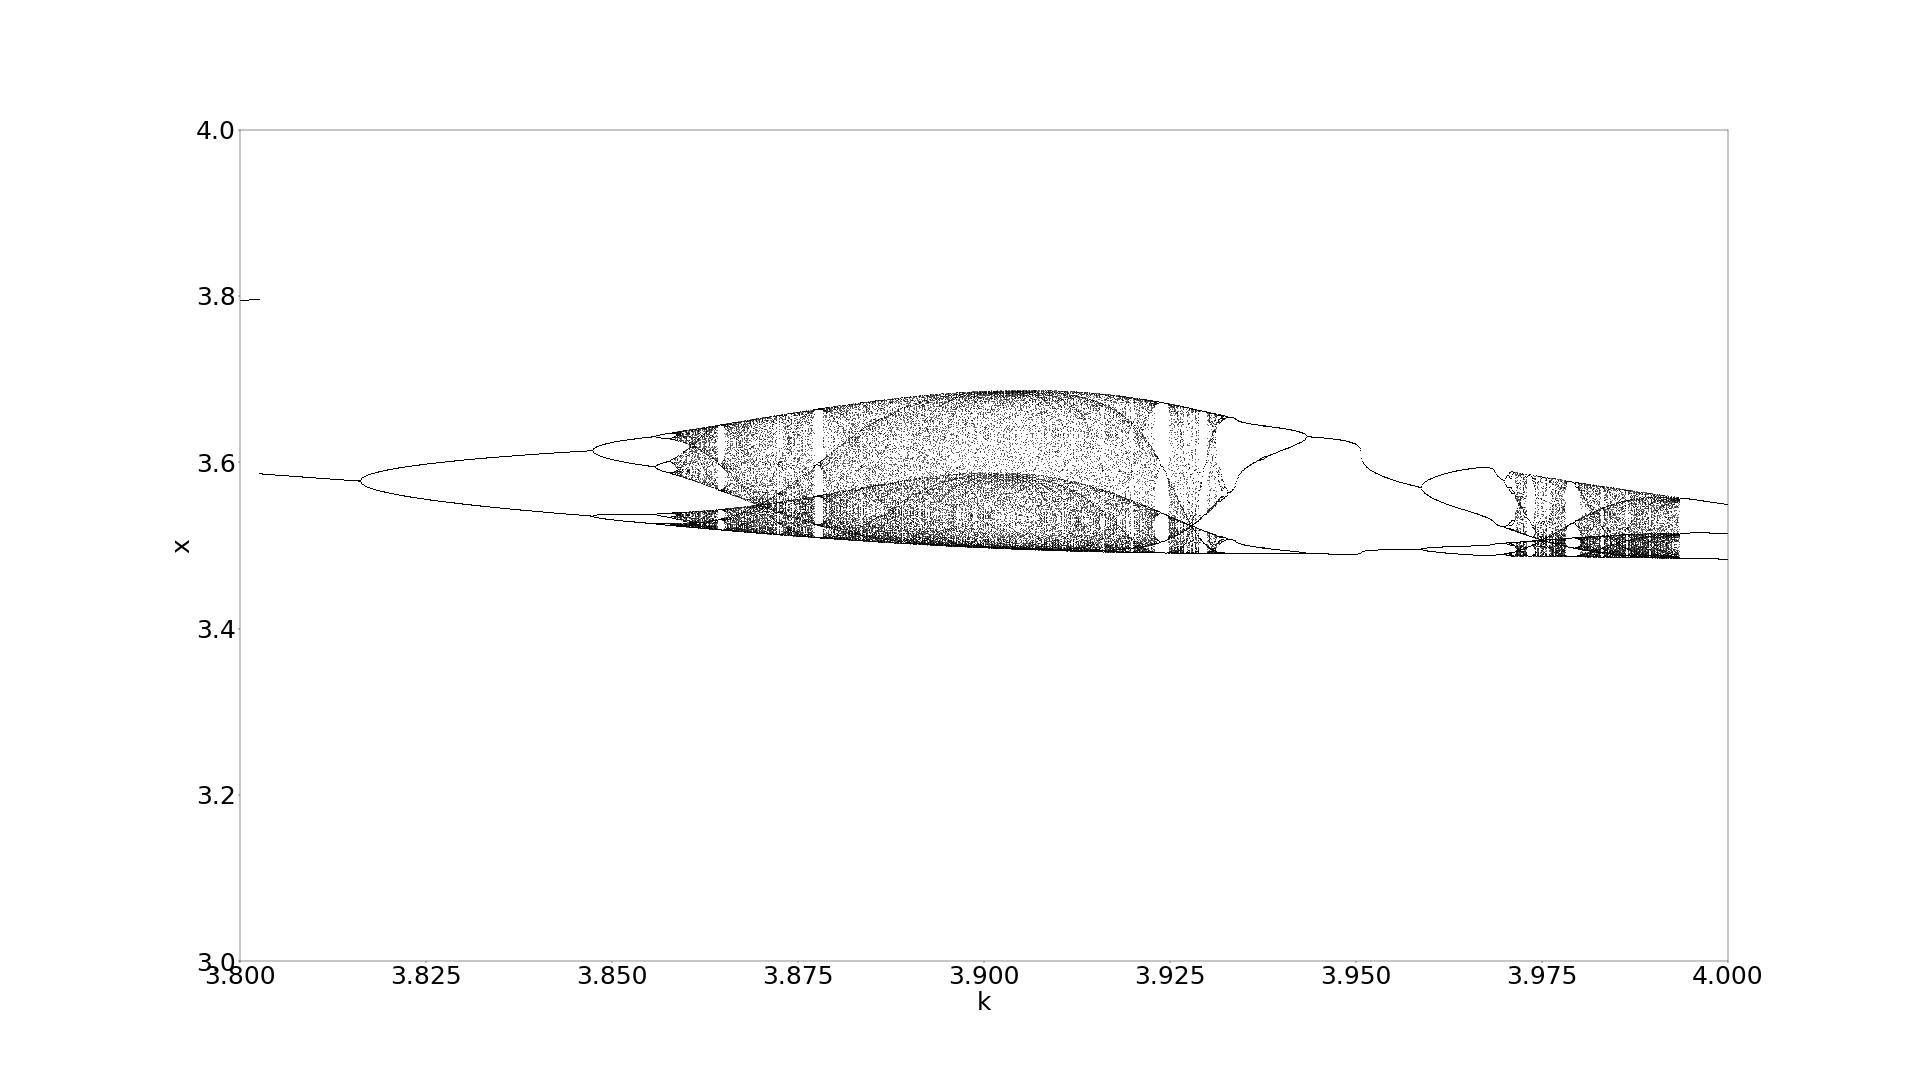
\includegraphics[width=\textwidth]{LateX images/sine q=-0.5/g12}
		\caption{$x_0=1$}
		\label{f:g533}
	\end{subfigure}
	
	\caption{Διαγράμματα διακλάδωσης για διάφορες τιμές του $x_0$. }
	\label{f:g237}
\end{figure}

\begin{figure}[ht]
	\centering
	
	\begin{subfigure}[b]{0.8\textwidth}
		\centering
		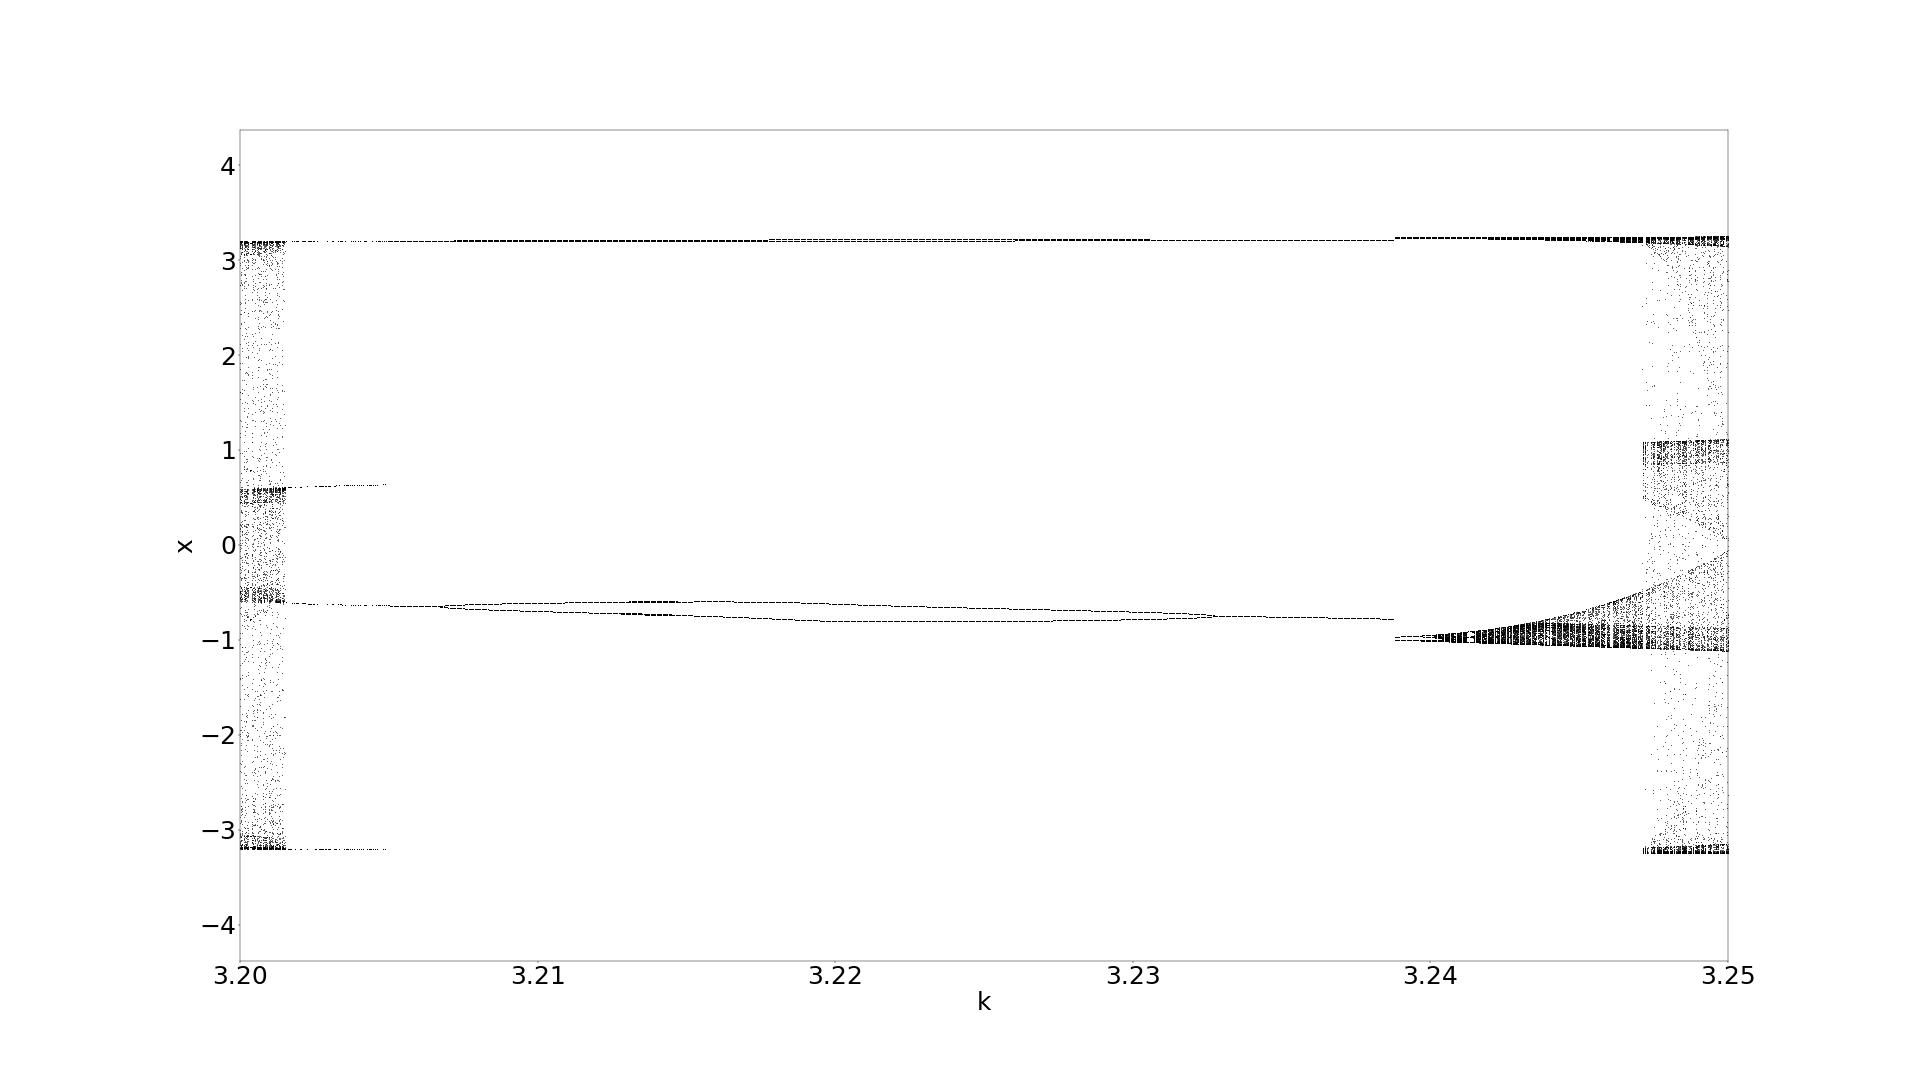
\includegraphics[width=\textwidth]{LateX images/sine q=-0.5/g2}
		\caption{$x_0=0.1$}
		\label{f:g54}
	\end{subfigure}
	\hfill
	\begin{subfigure}[b]{0.8\textwidth}
		\centering
		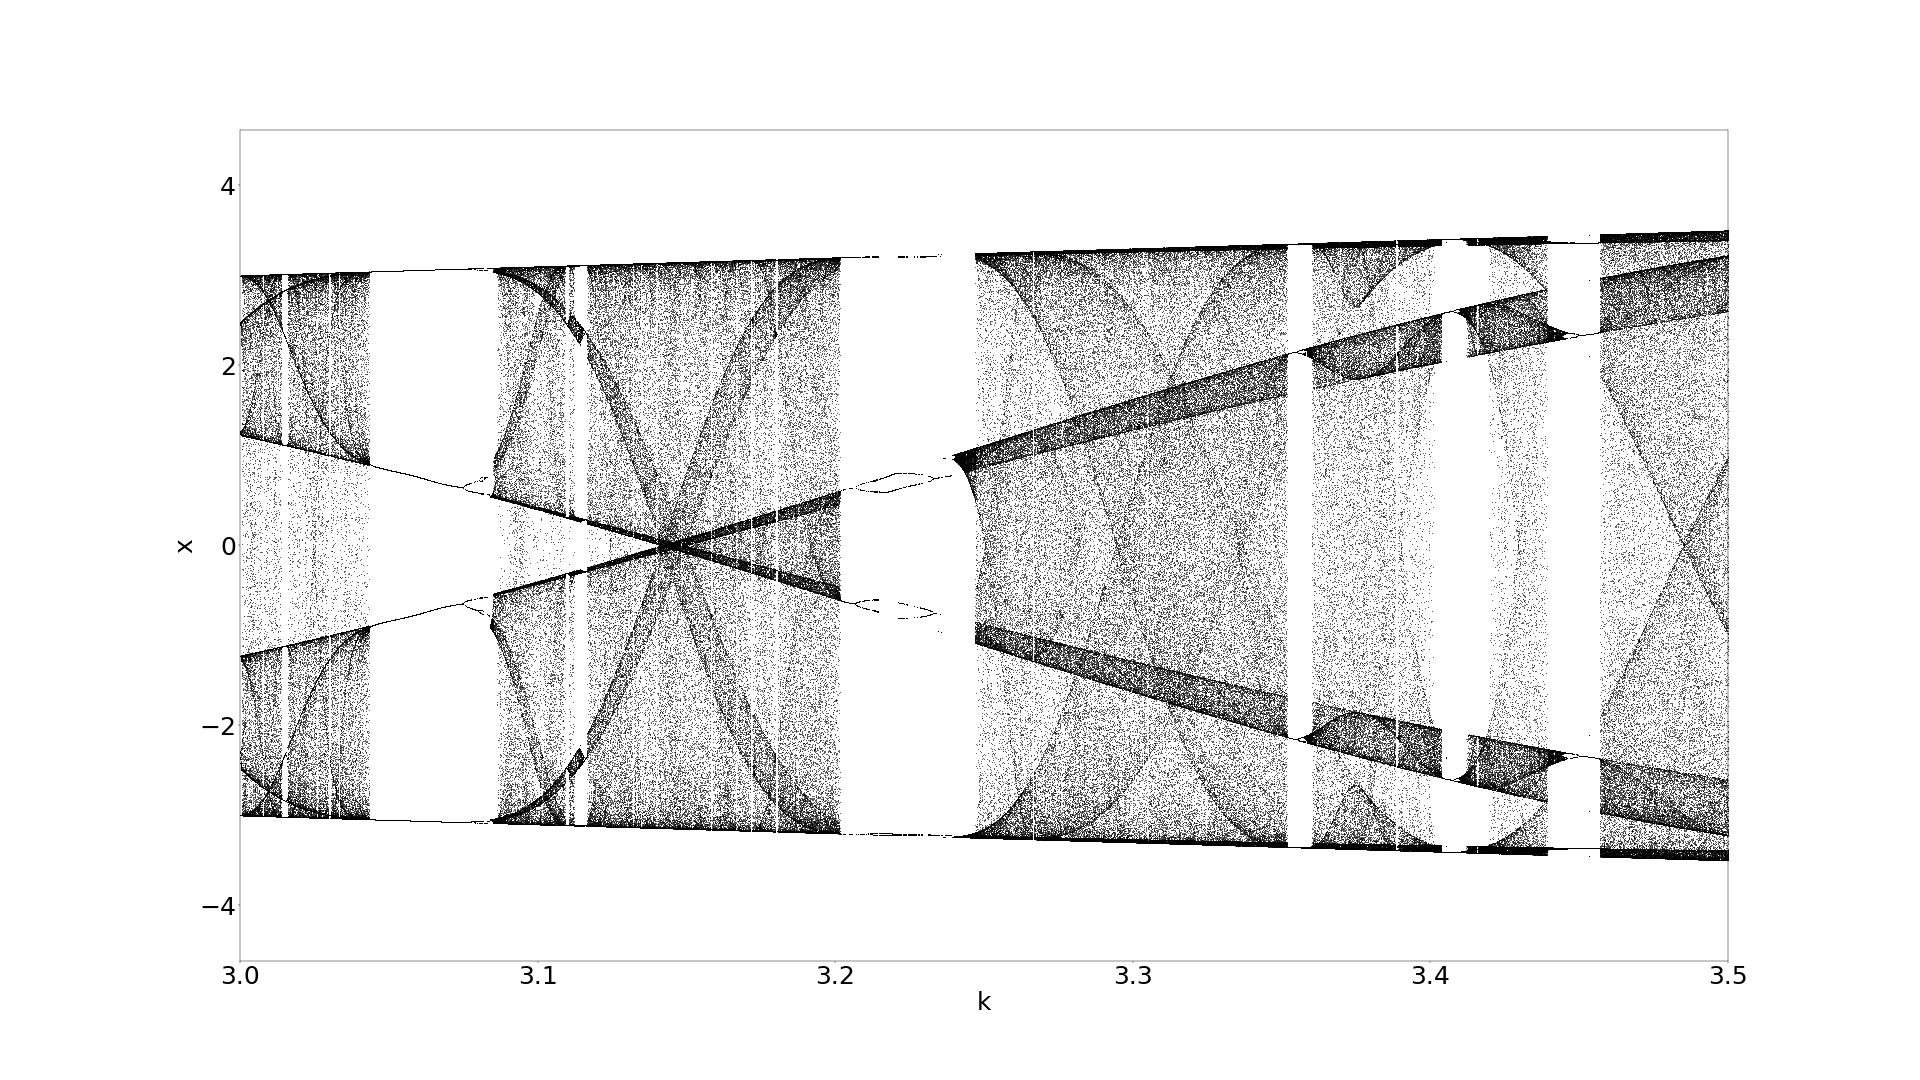
\includegraphics[width=\textwidth]{LateX images/sine q=-0.5/g14}
		\caption{$x_0=0.5$}
		\label{f:g55}
	\end{subfigure}
	\begin{subfigure}[b]{0.8\textwidth}
		\centering
		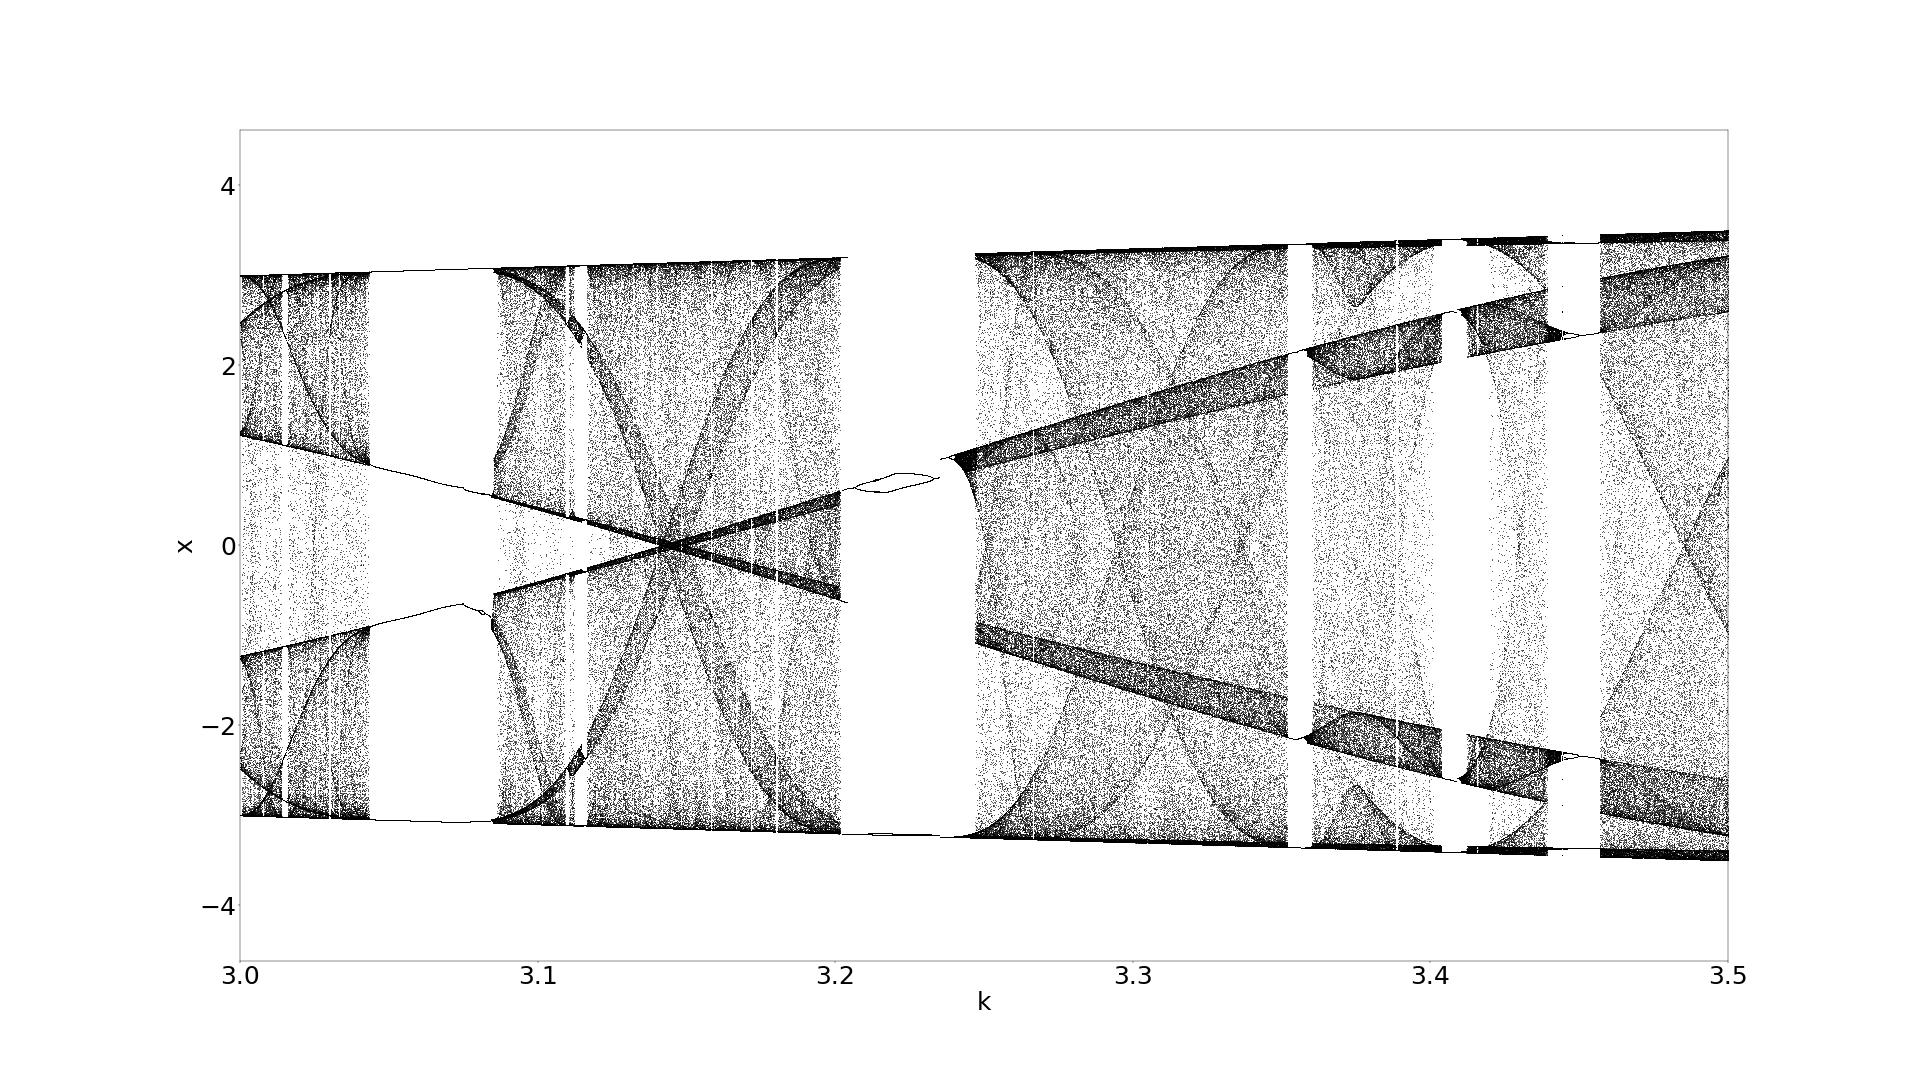
\includegraphics[width=\textwidth]{LateX images/sine q=-0.5/g15}
		\caption{$x_0=1$}
		\label{f:g56}
	\end{subfigure}
	
	\caption{Διαγράμματα διακλάδωσης για διάφορες τιμές του $x_0$. }
\end{figure}

\begin{figure}[ht]
	\centering
	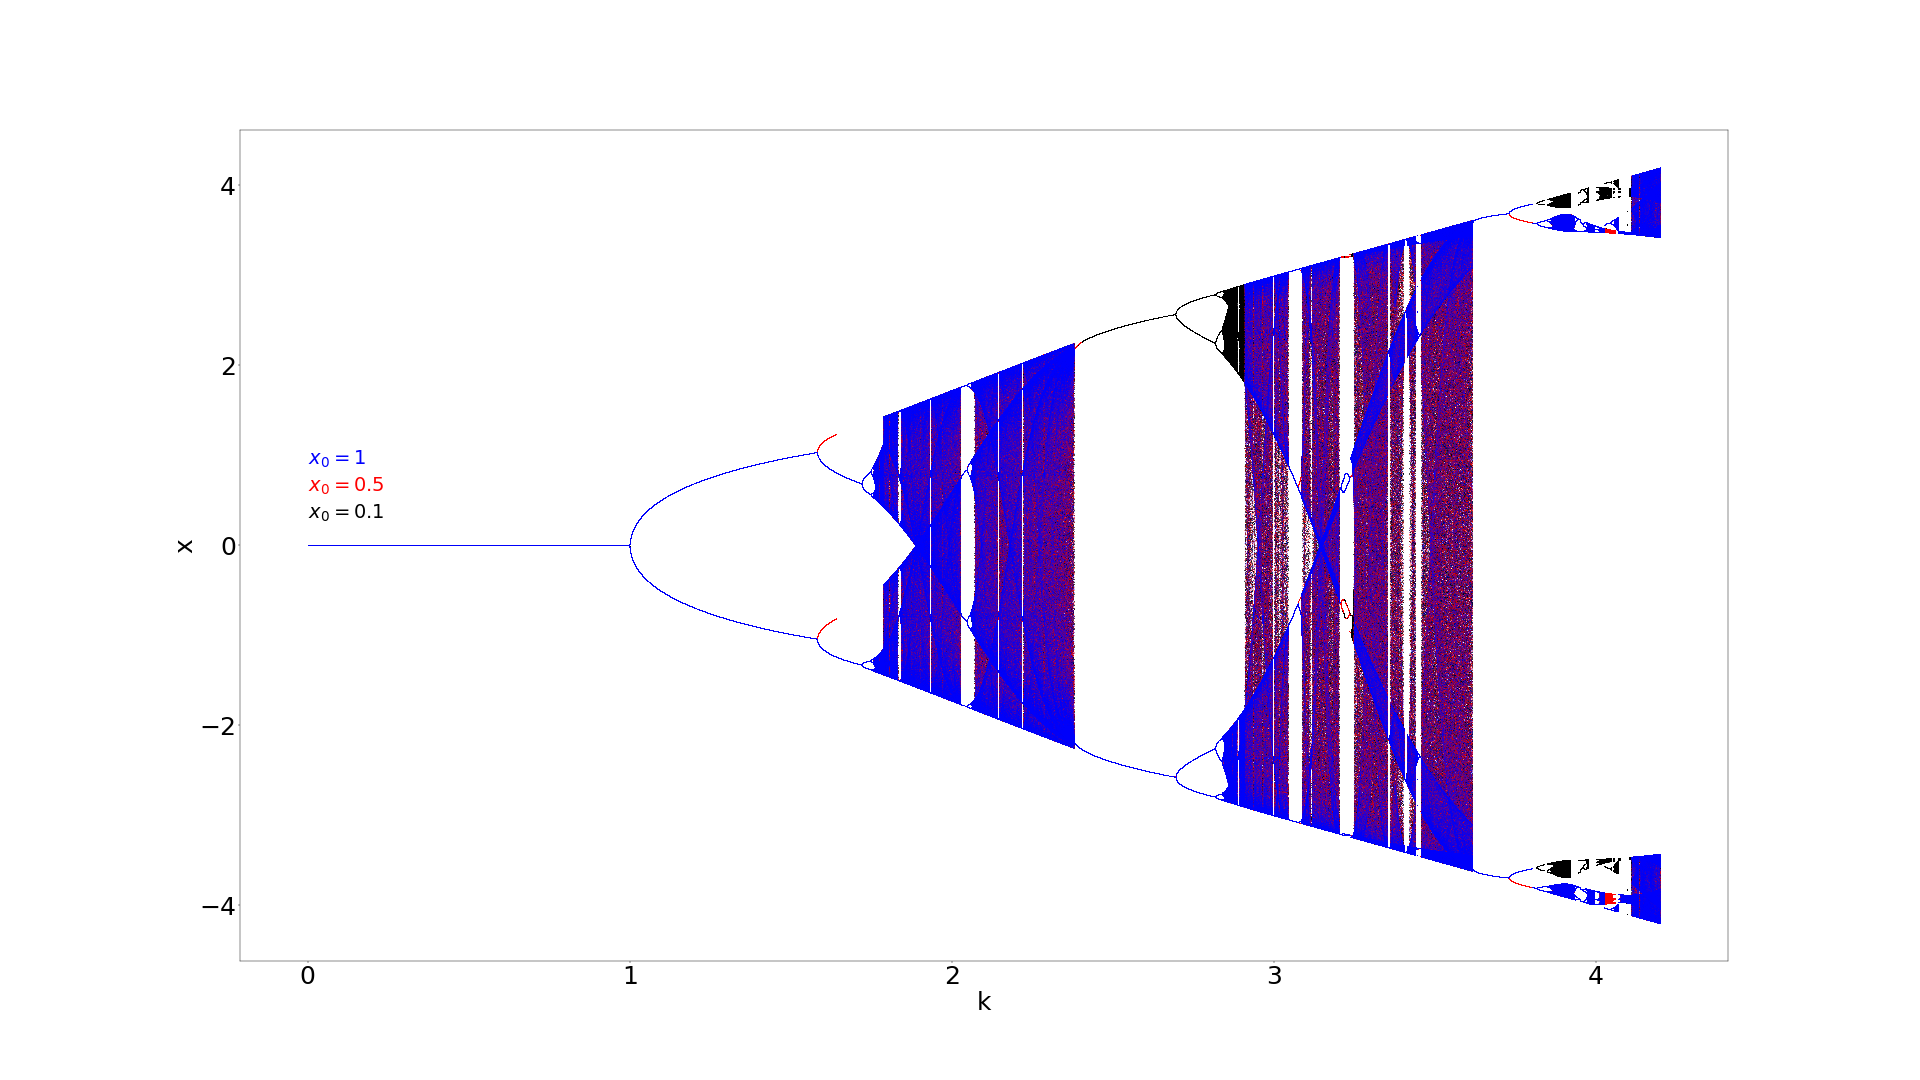
\includegraphics[width=1\linewidth]{LateX images/sine q=-0.5/g11}
	\caption{Διάγραμμα διακλάδωσης, για όλες τις διαφορετικές αρχικές συνθήκες $x_0$.}
	\label{f:g57}
\end{figure}

\begin{figure}[ht]
	\centering
	\begin{subfigure}[b]{0.4\textwidth}
		\centering
		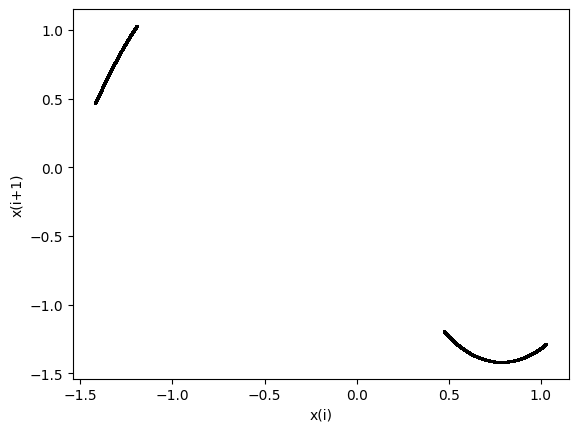
\includegraphics[width=\textwidth]{LateX images/sine q=-0.5/g16}
		\caption{Για $k=1.775$}
		\label{f:k127}
	\end{subfigure}
	\hfill
	\begin{subfigure}[b]{0.4\textwidth}
		\centering
		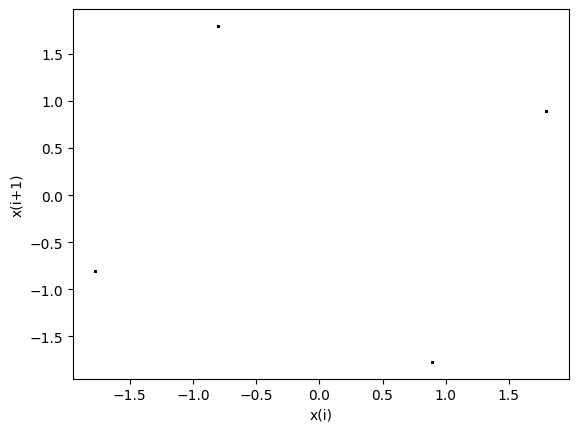
\includegraphics[width=\textwidth]{LateX images/sine q=-0.5/g17}
		\caption{Για $k=2.03$}
		\label{f:k128}
	\end{subfigure}
	\hfill
	\begin{subfigure}[b]{0.4\textwidth}
		\centering
		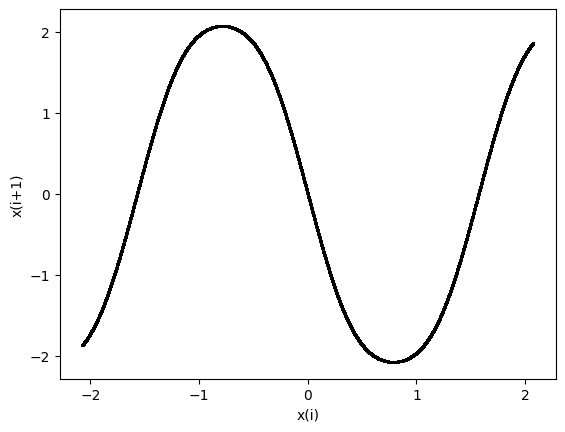
\includegraphics[width=\textwidth]{LateX images/sine q=-0.5/g19}
		\caption{Για $k=2.25$}
		\label{f:k129}
	\end{subfigure}
	\hfill
	\begin{subfigure}[b]{0.4\textwidth}
		\centering
		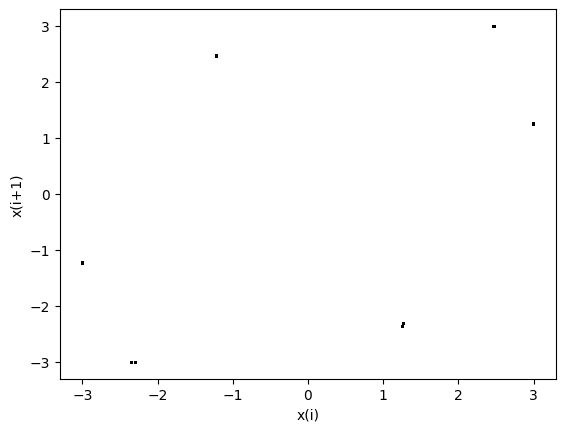
\includegraphics[width=\textwidth]{LateX images/sine q=-0.5/g18}
		\caption{Για $k=3$}
		\label{f:k130}
	\end{subfigure}
	\hfill
	\begin{subfigure}[b]{0.4\textwidth}
		\centering
		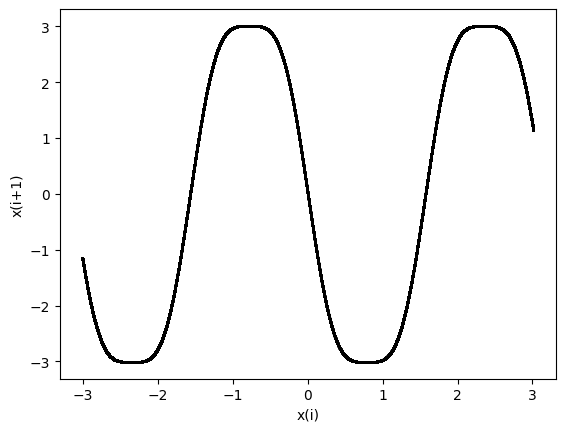
\includegraphics[width=\textwidth]{LateX images/sine q=-0.5/g20}
		\caption{Για $k=3.01$}
		\label{f:k131}
	\end{subfigure}
	\hfill
	\begin{subfigure}[b]{0.4\textwidth}
		\centering
		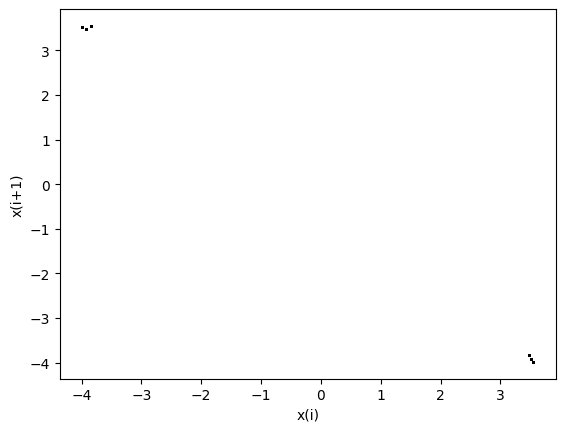
\includegraphics[width=\textwidth]{LateX images/sine q=-0.5/g21}
		\caption{Για $k=4$}
		\label{f:k132}
	\end{subfigure}
	\hfill			
	\caption{Διαγράμματα της τιμής \(x_i\) σε συνάρτηση με την τιμή \(x_{i+1}\) (α' μέρος).}
	\label{f:g58}
\end{figure}

\clearpage

\section{Συμπεράσματα}

Σε αυτό το κεφάλαιο παρουσιάστηκε μία παραλλαγή του \emph{sine-sinh-sine} Χάρτη, της οποίας βασικό χαρακτηριστικό είναι η χαοτική συμπεριφορά που εμφανίζε σε όλες τις περιπτώσεις που ελέχθηκαν για την παράμετρο \emph{q}, όπως και για τα επι μερούς φαινόμενα που οδηγούν σε αυτήν.

Ειδικότερα, το συνηθέστερο φαινόμενο που παρατηρήθηκε σε όλες τις περιπτώσεις είναι αυτό της μετάβασης στο χάος μέσω του διπλασιασμού της περιόδου, ξεκινώντας απο διάστημα \emph{περιόδου-1}.
Για κάποιες παραμέτρους  \emph{q} εμφανίστηκε η ανάστροφη πορεία του συστήματος κατά την έξοδο του απο την χαοτική περιοχή, παρουσιάζοντας έτσι το φαινόμενο της αντιμονοτονικότητας(χαοτική φυσαλίδα).
Επίσης αρκετές φορές παρατηρήθηκε το φαινόμενος της υστέρησης δηλαδή "έσπαγε" η περιοδική συμπεριφορά, καθώς και το φαινόμενο των κρίσεων είτε εσωτερικών που χαρακτηρίζονται από την διεύρηνση του χαοτικού τμήματος, είτε συνοριακές όπου το σύστημα εξέρχεται απότομα απο την χαοτική περιοχή και μεταβαίνει σε μία περιοδική.Παρατηρήθηκε οτι με  την δεύτερη μετέβαινε το σύστημα σε δίαστημα \emph{περιόδου-3}.